% Two-column, IEEE-Transactions-style layout. For the final submission replace the
% class/preamble by \documentclass[journal]{IEEEtran}; the sections are compatible.
\documentclass[10pt,twocolumn,a4paper]{article}
\usepackage[margin=0.75in,columnsep=0.25in]{geometry}
\usepackage[T1]{fontenc}
\usepackage[utf8]{inputenc}
\usepackage[expansion=false]{microtype}
\usepackage{booktabs,array,xcolor,amsmath,amssymb,graphicx,caption,float,enumitem,multirow,titlesec,stfloats}
\usepackage[numbers,sort&compress]{natbib}
\usepackage[colorlinks=true,linkcolor=blue!50!black,citecolor=blue!50!black,urlcolor=blue!50!black]{hyperref}
\captionsetup{font=footnotesize,labelfont=bf,labelsep=period,skip=3pt}
\setlength{\bibsep}{0pt}\setlength{\itemsep}{0pt}\renewcommand{\bibfont}{\scriptsize}
% IEEE-like headings
\renewcommand{\thesection}{\Roman{section}}
\renewcommand{\thesubsection}{\thesection.\Alph{subsection}}
\titleformat{\section}{\centering\normalfont\small\scshape}{\thesection.}{0.6em}{}
\titleformat{\subsection}{\normalfont\small\itshape}{\thesubsection}{0.6em}{}
\titlespacing*{\section}{0pt}{10pt}{5pt}\titlespacing*{\subsection}{0pt}{7pt}{3pt}
\setlength{\parskip}{0pt}\setlength{\parindent}{1em}
% ---- macros --------------------------------------------------------------
% ---- model names (always written out in full) ------------------------------
\usepackage{xspace}
\usepackage{algorithm}\usepackage{algpseudocode}
\algrenewcommand\algorithmicrequire{\textbf{Input:}}\algrenewcommand\algorithmicensure{\textbf{Output:}}
\newcommand{\MTN}{MTN\xspace}
\newcommand{\CAMTN}{PACE-Net without SATIE\xspace}
\newcommand{\CAMTNS}{PACE-Net\xspace}
\newcommand{\DFMTN}{PACE-Net with ROUTE\xspace}
\newcommand{\DFMTNS}{PACE-Net with ROUTE and SATIE\xspace}
\newcommand{\ESAS}{encoder self-attention sharing\xspace}
% ---- verification markers: set \drafttrue to show unresolved items in red ----
\newif\ifdraft \draftfalse
\newcommand{\verify}[1]{\ifdraft\textcolor{red}{\textbf{[verify: #1]}}\fi}
\DeclareMathOperator{\LN}{LN}\DeclareMathOperator{\MHA}{MHA}\DeclareMathOperator{\FFN}{FFN}
\DeclareMathOperator{\Drop}{Drop}\DeclareMathOperator{\Emb}{Emb}
\newcommand{\R}{\mathbb{R}}
\title{\vspace{-0.6em}\Large\bfseries PACE-Net: Admission-Gated Context Enrichment for Pedestrian Trajectory Prediction in Unstructured Traffic}
\author{\small Author names to be added\\[-2pt]\footnotesize Affiliation to be added}
\date{}
\begin{document}
\maketitle
\begin{abstract}
\noindent\textit{Abstract}---Predicting where a pedestrian will go in unstructured traffic is difficult because roads lack lane discipline and pedestrians are frequently occluded, yet most trajectory predictors reason only from motion cues such as bounding boxes, ego-vehicle speed and optical flow. This paper proposes PACE-Net (Pedestrian trajectory prediction with Admission-gated Context Enrichment), a new architecture for pedestrian trajectory prediction in unstructured traffic. The architecture has two pathways: a motion pathway that encodes boxes, speed and optical flow, and a context pathway in which a native scene-context encoder converts five static IDD-PeD scene attributes and the observed occlusion history into a single context token. Four components are proposed and evaluated: (i)~ROUTE (Routed Operator Unification of Trajectory and Environment), an adaptive context-memory fusion module that selects per sample how the context is merged with the trajectory memory; (ii)~SAGE (Sample-wise Admission Gate for Evidence), which decides per sample whether the context is used at all; (iii)~MASC (Memory Augmentation with Source-masked Context), in which the gated token is appended to the decoder memory and masked out of attention when rejected; and (iv)~SATIE (Self-Attention Tying in the Encoder), a selective weight-parameter sharing scheme that ties only the encoder self-attention projections across the three encoder layers and removes $6.07\%$ of the parameters. In a matched proof-of-concept study on IDD-PeD (fixed 32/8/24 split, three random seeds), PACE-Net obtained the lowest mean squared error (1080.2, compared with 1137.1 for the same architecture without sharing, a $5.0\%$ reduction), whereas ROUTE and full encoder--decoder weight sharing did not help (the final configuration therefore uses SAGE and MASC together with SATIE). The improvement is not statistically significant with three seeds (paired $p=0.45$), and the protocol differs from the published benchmark, so the results are presented as evidence motivating full-scale validation rather than as a benchmark claim.
\par\smallskip\noindent\textit{Index Terms}---Pedestrian trajectory prediction, unstructured traffic, scene context, admission gating, adaptive fusion, transformer, weight sharing, IDD-PeD.
\end{abstract}
\section{Introduction}\label{sec:intro}
\paragraph{Background.} Road traffic injuries remain a major public-health problem: the World Health Organization estimates 1.19 million road-traffic deaths per year, of which pedestrians account for 274,000 deaths (23\%)~\citep{who2023road}. Automated driving systems and advanced driver-assistance systems (ADAS) must therefore interact safely with pedestrians, avoiding collisions and allowing crossings to take place without hesitation~\citep{iddped2025}. A central capability is the anticipation of pedestrian motion: a vehicle that can estimate where a pedestrian will be one to two seconds ahead can brake, steer or yield early, whereas a purely reactive system must respond after the pedestrian has already entered the vehicle's path. Pedestrian trajectory prediction, i.e.\ forecasting the future bounding boxes of a pedestrian from an egocentric (vehicle-mounted) view, is accordingly a core component of the perception-and-planning stack.

\paragraph{Problem context.} Most learning-based predictors have been developed and evaluated on datasets collected in structured traffic, such as PIE and JAAD, in which crosswalks, traffic signals and yielding behaviour regularise pedestrian motion~\citep{rasouli2019pie,iddped2025}. These conditions are not representative of many parts of the world. In unstructured traffic, pedestrians walk along carriageways, cross diagonally between moving vehicles, hesitate or change direction after beginning to cross, and share the road with a dense and heterogeneous mix of vehicles, often without signals or marked crossings~\citep{iddped2025}. The recently released IDD-PeD dataset captures such conditions in Indian traffic and reports that established trajectory predictors degrade markedly on it: the error of the Multimodal Transformer Network (MTN) increases by up to 1,208 mean-squared-error units relative to its error on PIE~\citep{iddped2025}. Reliable prediction in unstructured traffic therefore remains an open problem.

\paragraph{Challenges.} Three difficulties are especially relevant. First, the \emph{motion cues are weak and ambiguous}: when pedestrians hesitate, pause or change direction, the past trajectory of a bounding box carries little information about the intended path, so predictors that rely on box history, ego-vehicle speed and optical flow alone have limited evidence on which to base a forecast. Second, \emph{pedestrians are frequently occluded and the scene varies strongly}, which further degrades visual and motion evidence and makes the appearance of the scene a poor guide to behaviour. Third, \emph{scene knowledge exists but is not exploited}: datasets such as IDD-PeD annotate, for every pedestrian track, the intersection type, signalisation, road type, location type, motion direction and occlusion state~\citep{iddped2025}. These attributes distinguish, for example, a pedestrian waiting at a signalised junction from one walking along an undivided road, yet compact trajectory models such as MTN~\citep{yin2021mtn} do not use them. Methods that do combine behavioural cues with scene information typically rely on image-level features such as regions of interest or segmentation maps and on stochastic decoders, and are evaluated on structured-traffic benchmarks~\citep{rasouli2022pedformer,sharma2025dual}.

\paragraph{Motivation.} The availability of cheap, interpretable, native annotations motivates a lightweight use of scene context. Two practical questions arise. (i)~\emph{How should static context be injected into an attention model without disturbing the motion pathway that has already been learned, and without harming samples for which the context is uninformative?} A single context token that a gate may admit or reject for each sample offers a safe fallback to the original model. (ii)~\emph{Can the additional capacity be paid for by removing redundancy elsewhere in the network?} Compact attention-based predictors are small models trained on limited data, so additional modules increase the risk of over-fitting, while their stacked encoder layers repeat the same type of self-attention computation. Sharing parameters across layers reduces the parameter count and can act as a regulariser~\citep{dehghani2019universal,lan2020albert}, but tying entire layers is harmful when layers play different roles, so the question becomes which sub-modules can be tied safely. Finally, because the study concerns small differences between closely related models, a controlled comparison under one protocol, with several seeds, is needed to separate genuine effects from run-to-run variation.

\paragraph{Approach and contributions.} This paper proposes PACE-Net, short for \emph{Pedestrian trajectory prediction with Admission-gated Context Enrichment} (Fig.~\ref{fig:overall}), a new architecture for pedestrian trajectory prediction in unstructured traffic. Its design rests on a separation of concerns: a \emph{motion pathway} models how the pedestrian moves, a \emph{context pathway} describes where the pedestrian is, and the two are merged only at the decoder memory, under the control of a learned admission gate. PACE-Net is built from four named components, which constitute the contributions of this paper.
\begin{itemize}[leftmargin=1.4em,itemsep=1pt,topsep=2pt]
\item \textbf{ROUTE (Routed Operator Unification of Trajectory and Environment).} An adaptive context-memory fusion module in which a selector chooses, for each sample, among three ways of merging scene context with the trajectory memory (identity, additive broadcast and cross-attention), so that the fusion strategy itself is learned (Sec.~\ref{ssec:fusion}).
\item \textbf{SAGE (Sample-wise Admission Gate for Evidence).} A hard, per-sample gate trained with a straight-through Gumbel-softmax decides whether the scene context is used at all, with the motion-only prediction as an exact fallback (Sec.~\ref{ssec:gate}).
\item \textbf{MASC (Memory Augmentation with Source-masked Context).} The gated 32-D native scene-context token, built from five IDD-PeD scene labels and the observed occlusion history, is appended to the decoder memory ($15\!\to\!16$ tokens) and masked out of attention when rejected (Sec.~\ref{ssec:memory}).
\item \textbf{SATIE (Self-Attention Tying in the Encoder).} A selective weight-parameter sharing scheme in which only the self-attention projections $(W_Q,W_K,W_V,W_O)$ of the three encoder layers are tied, reducing the parameter count by $6.07\%$ while all other modules remain layer-specific (Sec.~\ref{ssec:c4}).
\end{itemize}
These components are embedded in a dual-pathway architecture with its own design rationale (Sec.~\ref{ssec:rationale}) and are evaluated in a controlled, matched study, including a $2{\times}2$ factorial comparison of the two context-integration strategies with and without sharing, with per-seed numbers and paired statistics. In that study, ROUTE did not improve over the SAGE-gated token, and the final configuration therefore combines SAGE, MASC and SATIE; the negative result is reported openly.
The experiments constitute a proof-of-concept study (24 test trajectories, one training epoch, Farneb\"ack optical flow). The best model, \CAMTNS, has the lowest mean error and the fewest parameters, but its advantage over \CAMTN is within seed variance. The study is therefore reported as evidence for further validation and not as a benchmark result. The remainder of the paper is organised as follows: Section~\ref{sec:related} reviews related work, Section~\ref{sec:method} presents the method, Section~\ref{sec:results} the experiments, Section~\ref{sec:ablation} the ablation study, and Section~\ref{sec:limits} the limitations and conclusions.

\section{Related Work}\label{sec:related}
This section traces how pedestrian trajectory prediction has developed, identifies the limitations that remain in unstructured traffic, and states how each proposed component responds to them. The limitations are numbered L1--L4 and are summarised against the contributions in Table~\ref{tab:gaps}.

\subsection{From Social Models to Egocentric Prediction}
Early learning-based predictors treated a pedestrian as a sequence and modelled interaction between pedestrians. Social LSTM~\citep{alahi2016social} pooled the hidden states of neighbouring pedestrians, Social GAN~\citep{gupta2018socialgan} added adversarial training to produce several plausible futures, Social-STGCNN~\citep{mohamed2020stgcnn} replaced pooling by spatio-temporal graph convolutions, and Trajectron++-style models~\citep{salzmann2020trajectron} extended the generative formulation to heterogeneous agents. These models were developed for a fixed, bird's-eye view in which the positions of all agents are available, and their strength lies in modelling social interaction. They are not designed for an \emph{egocentric} setting, where a vehicle-mounted camera observes a pedestrian whose bounding box is influenced by the vehicle's own motion. Egocentric benchmarks, namely JAAD~\citep{rasouli2017jaad} and PIE~\citep{rasouli2019pie}, therefore added ego-vehicle speed and, later, optical flow as inputs, and PIE introduced a joint intention and trajectory baseline (PIETraj) built on recurrent networks. Surveys of the area~\citep{rasouli2020survey} note that the interaction between vehicle and pedestrian, and not only pedestrian--pedestrian interaction, is what matters for driving.

\textbf{Remaining limitation (L1).} Both families were developed and evaluated on data from structured traffic. When IDD-PeD was released, the error of established predictors on it was markedly higher than on PIE~\citep{iddped2025}, which indicates that cues that suffice under lane discipline, signals and crosswalks are insufficient when pedestrians walk along the carriageway, cross diagonally and hesitate.

\subsection{Transformer and Goal-Conditioned Predictors}
Attention-based models replaced recurrence to capture longer dependencies. Transformer forecasters for trajectories~\citep{giuliari2021transformer} and socio-temporal transformers such as AgentFormer~\citep{yuan2021agentformer} showed that self-attention is competitive with recurrent models. For egocentric prediction, MTN~\citep{yin2021mtn} used a multimodal transformer over bounding boxes, ego speed and optical flow with a deterministic decoder, and this combination is the strongest purely deterministic baseline reported on IDD-PeD~\citep{iddped2025}. A second line of work reduces uncertainty about the intended destination: endpoint-conditioned prediction~\citep{mangalam2020pecnet}, BiTraP~\citep{yao2021bitrap} with bidirectional goal estimation and SGNet~\citep{wang2022sgnet} with stepwise goal prediction. These stochastic models report the best of several sampled trajectories and obtain much lower errors on IDD-PeD than the deterministic models (Table~\ref{tab:prior})~\citep{iddped2025}, but best-of-$K$ numbers measure the quality of a set of hypotheses rather than of a single committed forecast, and the downstream planner still has to choose among them.

\textbf{Remaining limitation (L2).} Compact deterministic transformers rely on motion evidence alone. When a pedestrian pauses or changes direction, the motion history carries little information about the intended path, and no additional evidence about the \emph{situation} of the pedestrian is available to the model. Goal-conditioned methods address this by sampling several futures, not by supplying more evidence about the scene.

\subsection{Scene Context for Pedestrian Behaviour}
A natural response is to add scene context. Stacked recurrent models fused several contextual features for action anticipation, PedFormer~\citep{rasouli2022pedformer} modulates cross-modal attention and learns intention and trajectory jointly with gated multitask learning, and the dual-task model of Sharma et al.~\citep{sharma2025dual} fuses pedestrian regions of interest, scene attributes and past trajectories, refines cross-modal features with a progressive denoising attention module, trains with counterfactual manipulation of regions and segmentation maps, and predicts trajectories with a conditional variational autoencoder. These systems show that context helps for crossing intention and trajectory prediction. They also share three properties: context is injected by \emph{image-level features} (regions of interest, segmentation maps) that require an additional perception network; it is injected \emph{unconditionally}, so an uninformative or noisy context influences every sample; and the evaluation is on PIE and JAAD, i.e.\ structured traffic.

\textbf{Remaining limitation (L3).} It is not established how \emph{lightweight, native annotations} such as the intersection type, signalisation, road type, location type, motion direction and occlusion state provided by IDD-PeD can be injected into a compact attention model (i)~without altering the motion representation that is already learned and (ii)~without harming samples for which the context is uninformative. Context that cannot be switched off is a liability precisely in unstructured scenes, where the same label (for example an unsignalised junction) may or may not matter.

\subsection{Adaptive Fusion and Gating}
Selecting among computations per input has a long history in conditional computation. Hard and soft gates choose experts in sparsely-gated mixtures~\citep{shazeer2017moe}; discrete decisions are made trainable by the Gumbel-softmax relaxation~\citep{jang2017gumbel} and straight-through estimators~\citep{bengio2013ste}; and dynamic multimodal fusion~\citep{xue2022dynmm} chooses among fusion operations for each input of a multimodal model. These ideas have, to the authors' knowledge, not been applied to the fusion of static scene labels with a trajectory memory in egocentric pedestrian prediction, and their benefit when the amount of training data is small is untested; in the present study adaptive fusion adds parameters (Sec.~\ref{ssec:fusion}) without reducing computation, since all candidates are evaluated before one is selected.

\textbf{Remaining limitation (L4).} A fusion mechanism for context needs a guaranteed way to fall back to the motion-only prediction, and it needs to be evaluated under a matched protocol to establish whether the extra flexibility pays off.

\subsection{Parameter Sharing and Compact Models}
Models for pedestrian prediction are deployed on vehicles with limited memory and are trained on small datasets, so parameter efficiency matters. Sharing weights across layers reduces the parameter count and can regularise training: Universal Transformers~\citep{dehghani2019universal} repeat a single layer and ALBERT~\citep{lan2020albert} shares parameters across all layers. These studies share \emph{whole layers} (or all sub-modules) in large language-understanding models. In a multimodal encoder with two interacting streams, layers play different roles: the self-attention refines the same representation at every depth, whereas the source and cross attention exchange information between streams whose content changes with depth. It is therefore unclear which sub-modules can be tied safely, and sharing everything can harm accuracy (Sec.~\ref{sec:ablation}).

\textbf{Remaining limitation (L5).} A compact multimodal predictor has no principled way to reduce its parameters, and adding a context pathway increases them further.

\subsection{Positioning of the Present Contributions}
Table~\ref{tab:gaps} relates each limitation to the component that addresses it. The proposed architecture is deterministic, so that the effect of scene context and of parameter sharing can be isolated from the effect of a stochastic decoder; it is positioned as complementary to goal-conditioned sampling and not as a replacement. Native annotations replace image-level context features (L3), SAGE and the source mask of MASC provide an exact fallback to the motion-only prediction (L3, L4), ROUTE supplies a learned choice of fusion operation that is evaluated under a matched protocol (L4), MASC lets every decoder layer read the context through the attention it already uses (L2, L3), and SATIE offsets the added parameters (L5). Whether these remedies are sufficient is a matter of evidence, and Secs.~\ref{sec:results} and~\ref{sec:ablation} report where they did and did not help.

\begin{table*}[t]
\centering
\caption{Limitations of earlier approaches in unstructured traffic and the proposed components that address them.}
\label{tab:gaps}
\scriptsize
\begin{tabular}{p{0.3cm}p{4.9cm}p{4.4cm}p{5.5cm}}
\toprule
 & Limitation of earlier approaches & Where it arises & Proposed response\\
\midrule
L1 & Developed on structured-traffic data; performance drops on IDD-PeD & Social models, PIETraj, MTN~\citep{iddped2025} & Evaluation on IDD-PeD with native, unstructured-traffic annotations\\
L2 & Motion-only evidence is weak when pedestrians hesitate or turn & Deterministic transformers~\citep{yin2021mtn}; goal sampling gives hypotheses, not evidence & Native scene-context token added to the decoder memory (MASC)\\
L3 & Context needs image-level features and is injected unconditionally & PedFormer, dual-task CVAE model~\citep{rasouli2022pedformer,sharma2025dual} & Native labels; SAGE admission gate with exact fallback through the source mask (MASC)\\
L4 & Fusion operation is fixed; no fallback; benefit of adaptivity untested & Fixed fusion; dynamic fusion in other domains~\citep{xue2022dynmm} & ROUTE, adaptive fusion evaluated in a matched $2{\times}2$ study\\
L5 & Parameter growth; unclear which sub-modules can be tied & Whole-layer sharing~\citep{dehghani2019universal,lan2020albert} & SATIE: sharing of encoder self-attention only ($-6.07\%$)\\
\bottomrule
\end{tabular}
\end{table*}

\section{Proposed Method}\label{sec:method}
\subsection{Problem Formulation}
Given the observed bounding boxes of a pedestrian over $T{=}15$ frames (0.5\,s at 30\,fps), $\mathbf{X}_{obs}\in\R^{15\times4}$ with $\mathbf{x}_t=(x_1,y_1,x_2,y_2)_t$, the ego-vehicle speed $\mathbf{v}\in\R^{15\times1}$, an ego-motion optical-flow descriptor $\mathbf{F}_{ego}\in\R^{28\times64}$ and a pedestrian optical-flow descriptor $\mathbf{F}_{ped}\in\R^{28\times9}$, the task is to predict the future boxes $\hat{\mathbf{Y}}\in\R^{45\times4}$ for the next 1.5\,s. IDD-PeD additionally provides, for every track, five static scene labels $\mathbf{s}=(s_{int},s_{sig},s_{road},s_{loc},s_{dir})$ (intersection type, signalisation, road type, location type, motion direction) and a per-frame occlusion state $\mathbf{o}\in\{0,1,2,3\}^{15}$.

\subsection{Overview and Major Components}
Fig.~\ref{fig:overall} shows the proposed PACE-Net. The motion inputs are embedded to width $d_{model}{=}32$ (Sec.~\ref{ssec:embed}); a three-layer trajectory encoder produces the trajectory memory $\mathbf{M}_{traj}\in\R^{15\times32}$ (Sec.~\ref{ssec:enc}); a scene-context encoder maps the native IDD-PeD attributes to context tokens and a context vector $\mathbf{c}\in\R^{32}$ (Sec.~\ref{ssec:ctx}); the context is merged into the decoder memory; and a three-layer decoder with three parallel attention sources predicts a residual $\Delta\mathbf{Y}\in\R^{45\times4}$ that is added to the last observed box $\mathbf{x}_T$ repeated 45 times (Sec.~\ref{ssec:dec}).

The design is defined by four major components, each presented in its own subsection with a dedicated figure:
\begin{enumerate}[leftmargin=1.6em,itemsep=1pt,topsep=2pt]
\item \textbf{ROUTE}, adaptive context-memory fusion (Sec.~\ref{ssec:fusion}, Fig.~\ref{fig:fusion}, Algorithm~\ref{alg:fusion}): the context is merged with the trajectory memory by one of three fusion operations (identity, additive, cross-attention) chosen per sample by a learned selector.
\item \textbf{SAGE}, the admission gating mechanism (Sec.~\ref{ssec:gate}, Fig.~\ref{fig:gating}, Algorithm~\ref{alg:gate}): a hard, per-sample gate decides whether the context enters the decoder at all.
\item \textbf{MASC}, memory augmentation (Sec.~\ref{ssec:memory}, Fig.~\ref{fig:gating}b, Algorithm~\ref{alg:gate}): the gated context token is appended to the trajectory memory ($15\to16$ tokens) and exposed to the decoder through a source mask.
\item \textbf{SATIE}, selective weight-parameter sharing (Sec.~\ref{ssec:c4}, Fig.~\ref{fig:sharing}, Algorithm~\ref{alg:share}): only the encoder self-attention projections are tied across layers.
\end{enumerate}
ROUTE, and SAGE with MASC, are two alternative ways of integrating context; both were implemented and evaluated, and the final selected configuration (Sec.~\ref{sec:results}) uses SAGE and MASC together with SATIE. Removing the context pathway and the four components leaves a motion-only configuration (133,700 parameters) that serves as the baseline in the experiments.

\begin{figure*}[t]
\centering
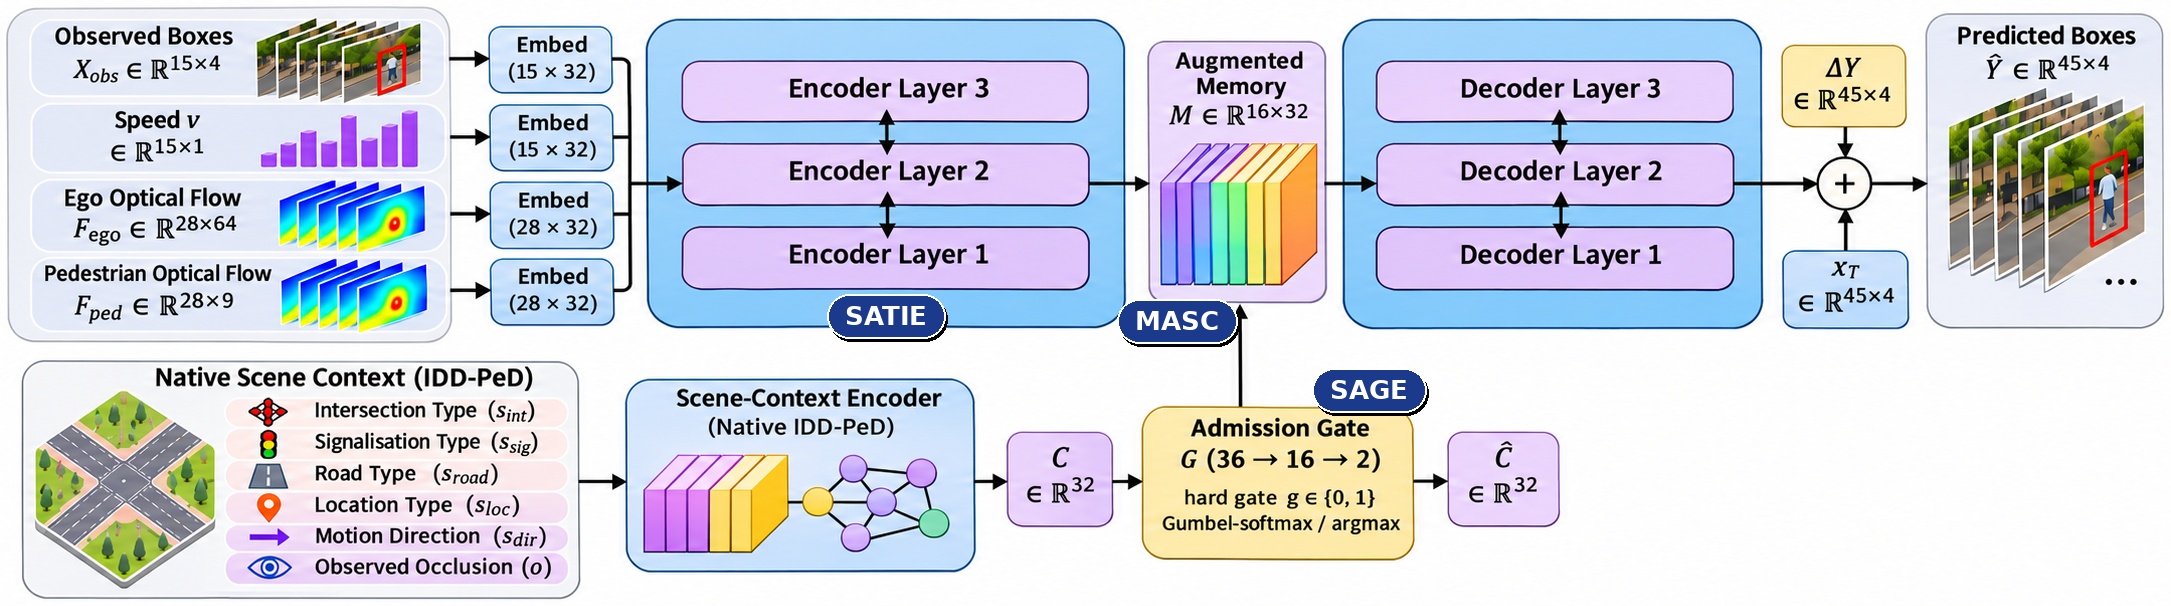
\includegraphics[width=0.97\textwidth]{figures/fig_overall.png}
\caption{Overall architecture of the proposed PACE-Net. Observed boxes and ego speed are embedded to $15{\times}32$ and processed by the three-layer trajectory encoder; the ego-flow and pedestrian-flow embeddings ($28{\times}32$) are consumed by the decoder through attention (Fig.~\ref{fig:decoder}). The five IDD-PeD scene labels and the observed occlusion are encoded into a 32-D context vector, a hard admission gate selects whether the token $\tilde{\mathbf{C}}$ is appended to the memory ($15{\to}16$ tokens), and the decoder output $\Delta\mathbf{Y}$ is added to the last observed box $\mathbf{x}_T$.}
\label{fig:overall}
\end{figure*}

\subsection{Design Rationale}\label{ssec:rationale}
The architecture is organised around five design principles, each of which addresses one of the challenges identified in Sec.~\ref{sec:intro}.
\begin{enumerate}[leftmargin=1.6em,itemsep=1pt,topsep=2pt]
\item \textbf{Separation of motion and context.} Motion evidence (boxes, speed, optical flow) is dynamic and changes at every frame, whereas scene attributes are static for a track. The two are therefore processed in separate pathways and are not mixed inside the encoder, so that the learned motion representation is left undisturbed by the context.
\item \textbf{Late fusion through the decoder memory.} The context pathway outputs a single token that is appended to the memory read by the decoder. Fusion at the memory costs only 5,442 additional parameters (4.07\% of the motion-only configuration) and lets every decoder layer query the context through the same attention mechanism that it uses for motion.
\item \textbf{Conditional admission with a guaranteed fallback.} Scene attributes are informative for some samples and not for others. A hard per-sample gate admits or rejects the token, and rejection removes the token from attention through the source mask, so the decoder then computes exactly what it would compute without context; the context branch can only be used or ignored, never forced.
\item \textbf{Native, interpretable context.} The context pathway consumes the attributes that IDD-PeD already annotates per track (Sec.~\ref{ssec:ctx}) instead of image-level features, which avoids an additional perception network and keeps each input interpretable.
\item \textbf{Selective redundancy removal.} The three encoder layers repeat the same self-attention computation, so only the self-attention projections are shared (Sec.~\ref{ssec:c4}). Source attention, cross attention, feed-forward networks and the decoder serve different roles at different depths and are kept layer-specific.
\end{enumerate}

\subsection{Multimodal Input Embedding}\label{ssec:embed}
Each modality is mapped to $d_{model}{=}32$ by a learned linear embedding, giving $\R^{15\times32}$ for boxes and speed and $\R^{28\times32}$ for the two flow streams (the first row of Fig.~\ref{fig:overall}). The trajectory embedding is followed by positional encoding. The ego and pedestrian flow descriptors use $8{\times}8{=}64$ and $3{\times}3{=}9$ spatial patches respectively, each with two flow channels.

\subsection{Dual-Stream Trajectory Encoder}\label{ssec:enc}
The motion pathway adopts the dual-stream attention block introduced in MTN~\citep{yin2021mtn}. The encoder has $N{=}3$ layers, $h{=}4$ heads, $d_{ff}{=}128$ and dropout $0.1$, and keeps two streams, a trajectory stream $\mathbf{x}$ and a speed-token stream $\mathbf{m}$, both in $\R^{15\times32}$ (Fig.~\ref{fig:encoder}). Layer $l$ computes
\begin{align}
\mathbf{x}' &= \mathbf{x}^{(l-1)} + \Drop\big(\MHA_{self}(\LN(\mathbf{x}^{(l-1)}))\big),\\
\mathbf{m}' &= \mathbf{m}^{(l-1)} + \Drop\big(\MHA_{src}(\LN(\mathbf{m}^{(l-1)}),\mathbf{x}')\big),\\
\mathbf{x}'' &= \mathbf{x}' + \Drop\big(\MHA_{cross}(\LN(\mathbf{x}'),\mathbf{m}')\big),
\end{align}
followed by feed-forward residual blocks that produce $(\mathbf{x}^{(l)},\mathbf{m}^{(l)})$. Source attention lets the speed stream read the trajectory, and cross attention lets the trajectory stream read the speed. The output of the last layer is the trajectory memory $\mathbf{M}_{traj}=\mathbf{x}^{(3)}\in\R^{15\times32}$.

\begin{figure*}[t]
\centering
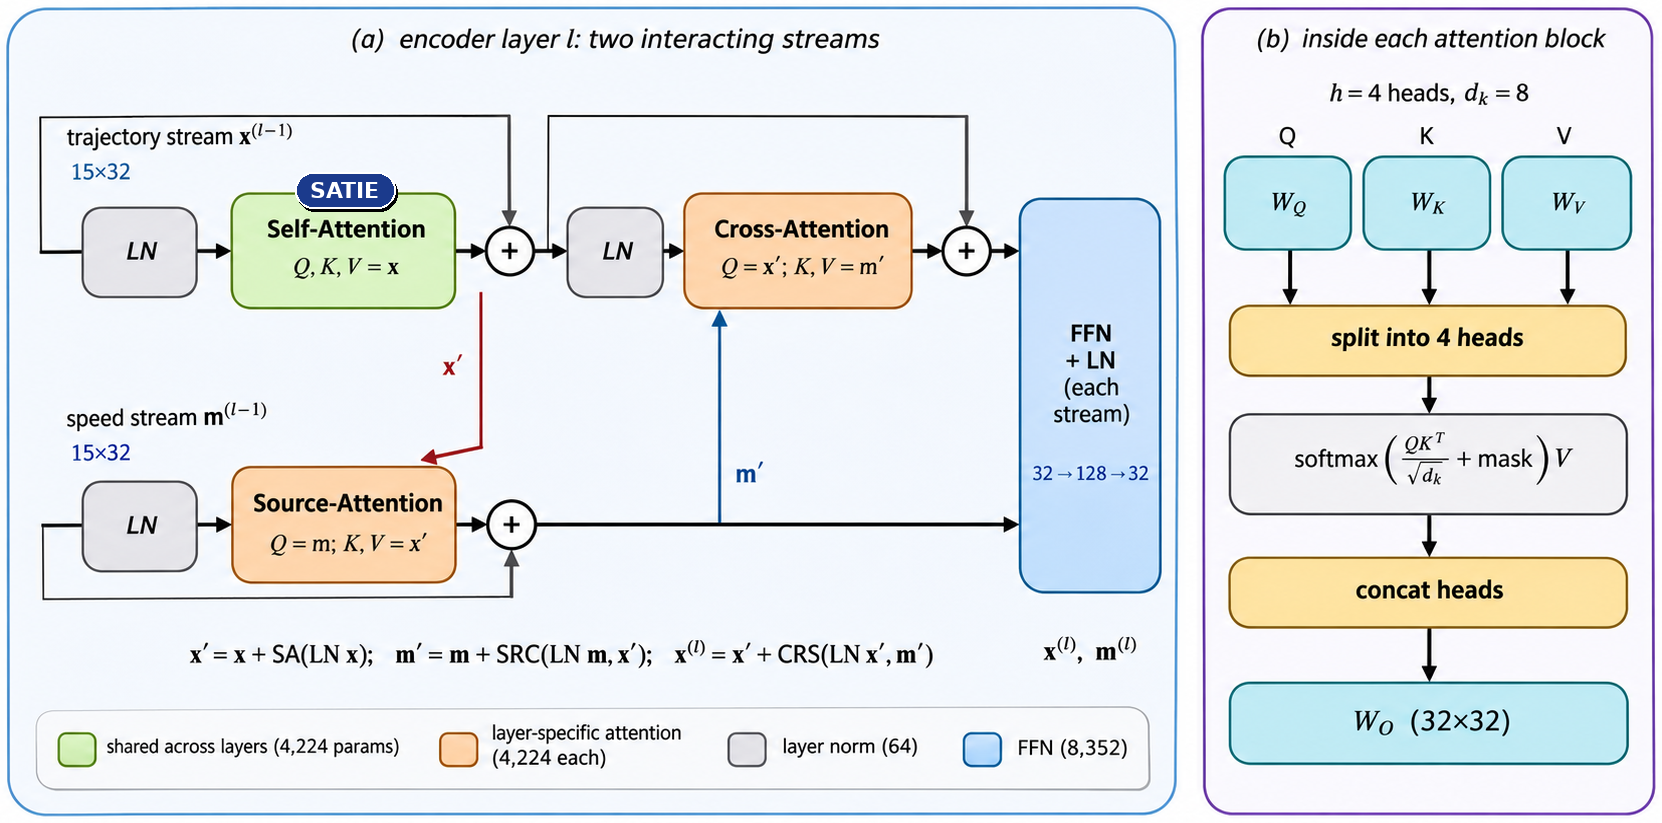
\includegraphics[width=0.85\textwidth]{figures/fig_enc_new.png}
\caption{Dual-stream trajectory encoder layer with shared self-attention. (a)~Layer $l$ updates a trajectory stream $\mathbf{x}$ and a speed stream $\mathbf{m}$ ($15{\times}32$ each) in four steps: self-attention on $\mathbf{x}$ (the module shared across layers, green), source attention in which $\mathbf{m}$ reads the updated trajectory $\mathbf{x}'$, cross attention in which $\mathbf{x}'$ reads the updated speed $\mathbf{m}'$ (both layer-specific, orange), and feed-forward residual blocks. Every sub-layer uses pre-layer-normalisation and a residual connection. (b)~Internal structure of every attention block: query, key and value projections, four heads ($d_k{=}8$), scaled dot-product attention with optional mask, head concatenation and output projection.}
\label{fig:encoder}
\end{figure*}

\subsection{Native Scene-Context Encoding Module}\label{ssec:ctx}
\paragraph{Motivation.} Box and flow history cannot tell whether a pedestrian is at a signalised junction or on an open road. IDD-PeD already annotates such attributes per track, so the proposed model uses them directly, without an additional perception model.

\paragraph{Encoder.} Each categorical field $s_k$, $k\in\{int,sig,road,loc,dir\}$, is embedded into $\R^{16}$ with a learnable table $E_k$ (Fig.~\ref{fig:context}). The observed occlusion sequence is embedded (4 states $\to$16) and mean-pooled over the 15 frames. The six 16-D vectors are concatenated ($6{\times}16{=}96$) and passed through a small MLP:
\begin{align}
\mathbf{u} &= \big[E_{int}(s_{int});\dots;E_{dir}(s_{dir});\ \tfrac1{15}\textstyle\sum_{t}E_{occ}(o_t)\big]\in\R^{96},\\
\mathbf{c} &= W_2\,\Drop\big(\mathrm{GELU}(W_1\,\LN(\mathbf{u})+b_1)\big)+b_2\in\R^{32},
\end{align}
with $W_1\in\R^{32\times96}$ (Fig.~\ref{fig:context}) and $W_2\in\R^{32\times32}$. The context encoder has 4,816 parameters. The fusion variant (Sec.~\ref{ssec:fusion}) additionally keeps the six 16-D vectors as separate tokens, projected to $\R^{6\times32}$ by a shared $16\to32$ layer. Only information available by the end of the observation window is used; time of day is deliberately excluded because it is not an annotated per-track attribute.

\begin{figure*}[t]
\centering
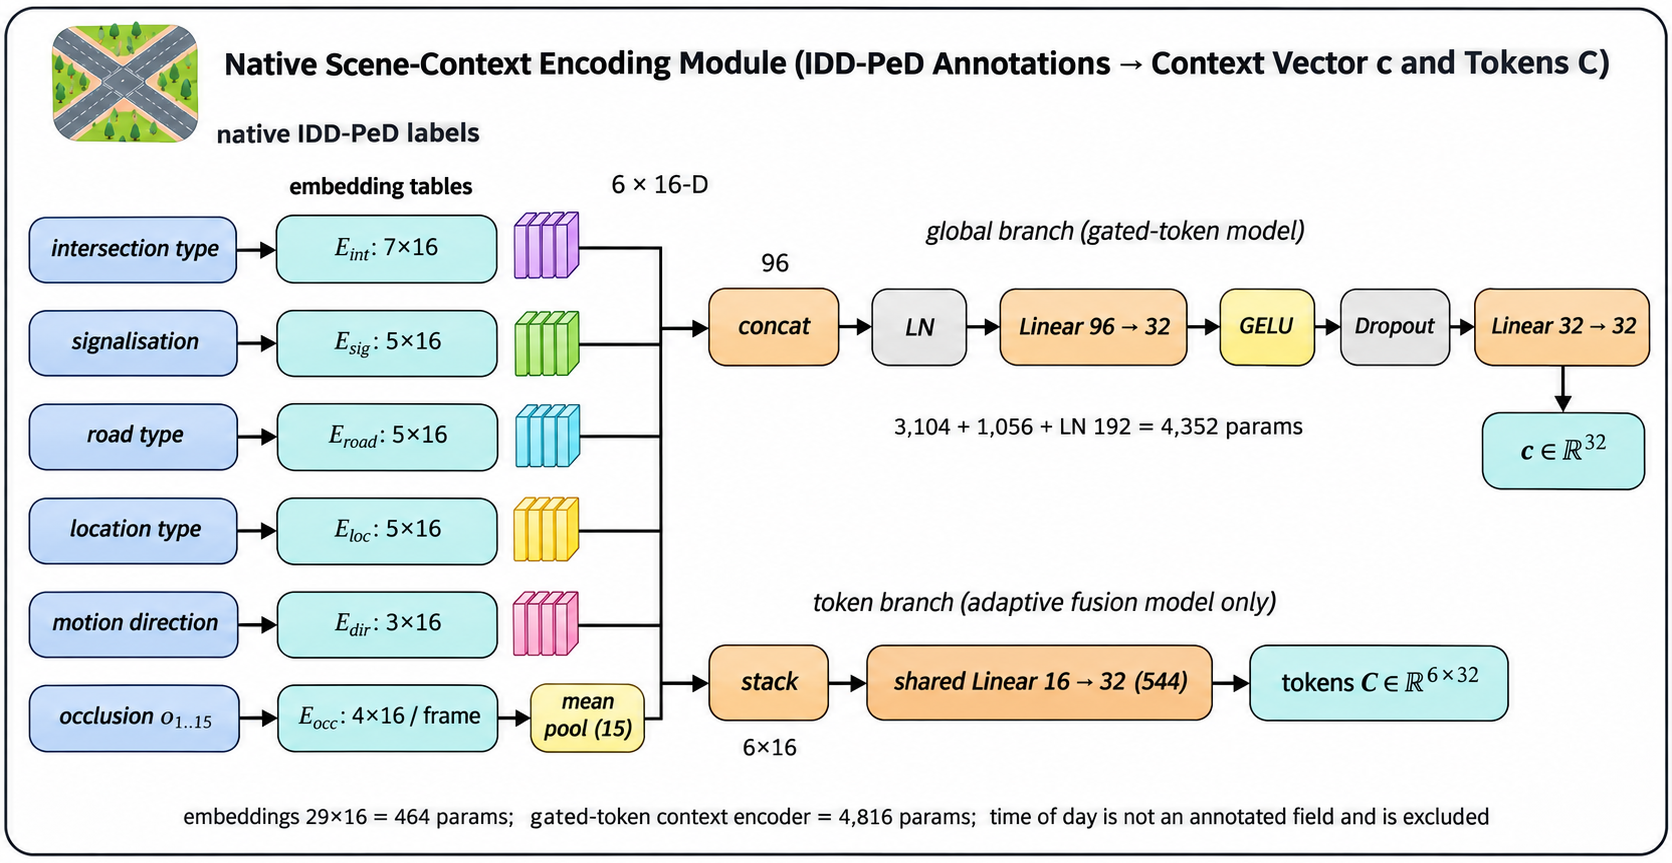
\includegraphics[width=0.85\textwidth]{figures/fig_context_new.png}
\caption{Native scene-context encoding module. Five categorical IDD-PeD labels (with vocabulary sizes 7, 5, 5, 5 and 3, each including an ``unknown'' value) and the 15-frame occlusion sequence (4 states, mean-pooled over time) are embedded to 16-D. The global branch concatenates the six vectors (96-D) and applies layer normalisation and a two-layer MLP to give the context vector $\mathbf{c}\in\R^{32}$ (4,816 parameters in total); the token branch, used only by the adaptive-fusion model, projects the six vectors to context tokens $\mathbf{C}\in\R^{6\times32}$.}
\label{fig:context}
\end{figure*}

\subsection{ROUTE: Routed Operator Unification of Trajectory and Environment}\label{ssec:fusion}
\paragraph{Motivation.} A fixed way of combining context with motion memory cannot suit every pedestrian: for some samples the memory alone suffices, for others a broadcast scene summary helps, and for others the memory should actively query individual scene attributes. ROUTE (Routed Operator Unification of Trajectory and Environment) lets the model choose, per sample, how the context is merged with the trajectory memory, in the spirit of dynamic multimodal fusion~\citep{xue2022dynmm}.

\paragraph{Mechanism.} Let $\mathbf{C}\in\R^{6\times32}$ be the six context tokens and $\mathbf{c}\in\R^{32}$ the global context vector (Sec.~\ref{ssec:ctx}). Three candidate fusions of the trajectory memory are formed (Fig.~\ref{fig:fusion}):
\begin{align}
\mathbf{O}_1&=\mathbf{M}_{traj}, \quad\text{(identity)}\\
\mathbf{O}_2&=\LN\big(\mathbf{M}_{traj}+\mathbf{1}\,\mathbf{c}^\top\big), \quad\text{(additive)}\\
\mathbf{Z}&=\LN\big(\mathbf{M}_{traj}+\MHA(\mathbf{M}_{traj},\mathbf{C},\mathbf{C})\big),\\
\mathbf{O}_3&=\LN\big(\mathbf{Z}+\FFN(\mathbf{Z})\big). \quad\text{(cross-attention)}
\end{align}
A selector
\begin{equation}\boldsymbol{\ell}=W_{s2}\,\mathrm{GELU}\big(W_{s1}[\bar{\mathbf{M}}_{traj};\mathbf{c}]\big)\in\R^{3}\end{equation}
with $W_{s1}\in\R^{32\times64}$ and mean-pooled memory $\bar{\mathbf{M}}_{traj}$ produces one-hot weights $\mathbf{w}$ (hard straight-through Gumbel-softmax in training, $\arg\max$ at inference), and the fused memory $\mathbf{M}_f=\sum_{i=1}^{3}w_i\mathbf{O}_i\in\R^{15\times32}$ replaces $\mathbf{M}_{traj}$ in the decoder (Algorithm~\ref{alg:fusion}). Compared with the motion-only configuration the module adds 20,307 parameters, and all three candidates are computed before selection, so it does not reduce computation.

\begin{figure*}[t]
\centering
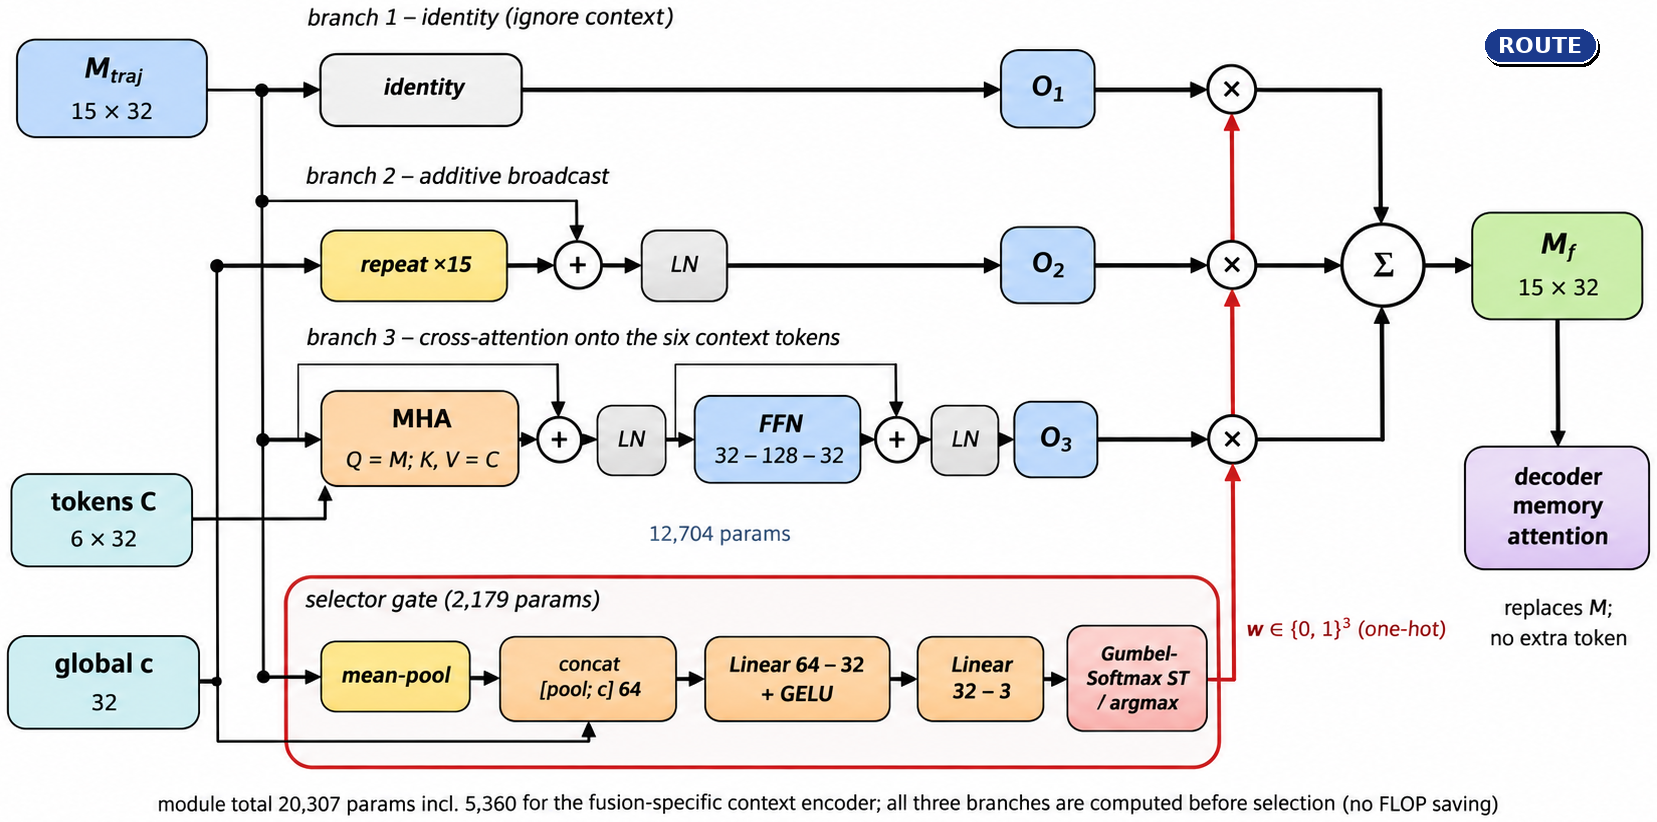
\includegraphics[width=0.85\textwidth]{figures/fig_fusion_new.png}
\caption{ROUTE, the adaptive context-memory fusion module (\textbf{1}). Three fusion operators act on the trajectory memory: identity (branch~1), additive broadcast of the global context followed by layer normalisation (branch~2), and cross-attention onto the six context tokens with a feed-forward block (branch~3). A selector gate on the pooled memory and the global context produces a one-hot weight vector $\mathbf{w}$ (straight-through Gumbel-softmax in training, $\arg\max$ at inference); the weighted sum $\mathbf{M}_f$ replaces the memory read by the decoder.}
\label{fig:fusion}
\end{figure*}

\begin{algorithm}[t]
\caption{ROUTE: adaptive context-memory fusion (forward pass)}\label{alg:fusion}
\begin{algorithmic}[1]
\Require trajectory memory $\mathbf{M}_{traj}\in\R^{15\times32}$, context tokens $\mathbf{C}\in\R^{6\times32}$, global context $\mathbf{c}\in\R^{32}$, mode $\in\{\text{train},\text{eval}\}$
\Ensure fused memory $\mathbf{M}_f\in\R^{15\times32}$
\State $\mathbf{O}_1\gets\mathbf{M}_{traj}$
\State $\mathbf{O}_2\gets\LN(\mathbf{M}_{traj}+\mathbf{1}\mathbf{c}^\top)$
\State $\mathbf{Z}\gets\LN(\mathbf{M}_{traj}+\Drop(\MHA(\mathbf{M}_{traj},\mathbf{C},\mathbf{C})))$
\State $\mathbf{O}_3\gets\LN(\mathbf{Z}+\Drop(\FFN(\mathbf{Z})))$
\State $\boldsymbol{\ell}\gets W_{s2}\,\mathrm{GELU}(W_{s1}[\mathrm{mean}(\mathbf{M}_{traj});\mathbf{c}])$
\If{mode $=$ train}
  \State $\mathbf{w}\gets$ one-hot(GumbelSoftmax$(\boldsymbol{\ell})$) with straight-through gradient
\Else
  \State $\mathbf{w}\gets$ one-hot$(\arg\max\boldsymbol{\ell})$
\EndIf
\State \Return $\sum_{i=1}^{3}w_i\,\mathbf{O}_i$
\end{algorithmic}
\end{algorithm}

\subsection{SAGE: Sample-wise Admission Gate for Evidence}\label{ssec:gate}
\paragraph{Motivation.} Context is not equally informative for every sample, and an uninformative token can distract the decoder. The gate gives the model an explicit, per-sample choice to use or ignore the context, with the motion-only prediction as a guaranteed fallback.

\paragraph{Mechanism.} The gate observes the context vector and the current motion state $\mathbf{x}_T$ (Fig.~\ref{fig:gating}a):
\begin{align}
\boldsymbol{\ell}&=W_{g2}\,\mathrm{GELU}\big(W_{g1}[\mathbf{c};\mathbf{x}_T]+b_{g1}\big)+b_{g2}\in\R^{2},\\
g&=\begin{cases}\text{one-hot}(\mathrm{GumbelSoftmax}(\boldsymbol{\ell}))_2 & \text{training},\\ \arg\max\boldsymbol{\ell} & \text{evaluation},\end{cases}
\end{align}
with $W_{g1}\in\R^{16\times36}$ and $W_{g2}\in\R^{2\times16}$ (626 parameters). The hard straight-through Gumbel-softmax~\citep{jang2017gumbel,bengio2013ste} makes the forward pass discrete while gradients flow through the soft relaxation, so the decision can be learned end to end. The gated token is $\tilde{\mathbf{c}}=g\,\mathbf{c}$.

\begin{figure*}[t]
\centering
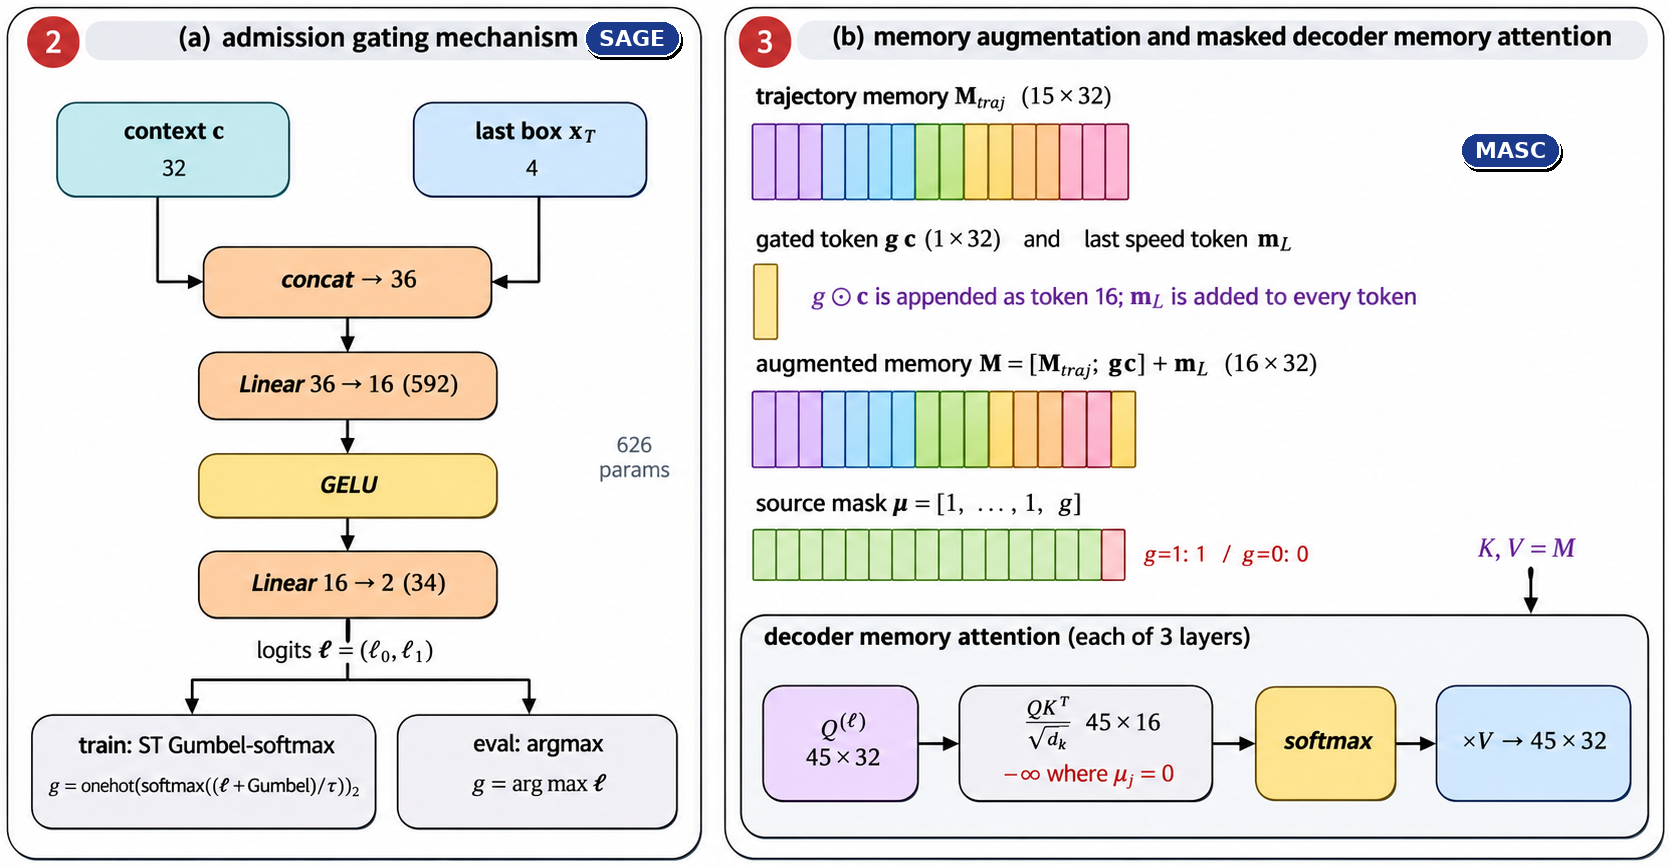
\includegraphics[width=0.85\textwidth]{figures/fig_gate_new.png}
\caption{SAGE admission gating (\textbf{2}) and MASC memory augmentation (\textbf{3}). (a)~The gate concatenates the context vector and last observed box (36-D), applies a two-layer network (626 parameters) and obtains a hard decision $g\in\{0,1\}$ by straight-through Gumbel-softmax (training) or $\arg\max$ (evaluation). (b)~The gated token is appended to the 15 trajectory-memory tokens (16 tokens) and $g$ forms the last entry of the source mask; inside the decoder memory attention, masked keys receive $-\infty$ scores, so a rejected token has zero attention weight.}
\label{fig:gating}
\end{figure*}

\subsection{MASC: Memory Augmentation with Source-masked Context}\label{ssec:memory}
The gated token is appended to the trajectory memory after the encoder (Fig.~\ref{fig:gating}b):
\begin{equation}
\mathbf{M}=\big[\mathbf{M}_{traj};\ g\,\mathbf{c}\big]+\mathbf{m}_L\in\R^{16\times32},\qquad \boldsymbol{\mu}=[\underbrace{1,\dots,1}_{15},\ g],
\end{equation}
where $\mathbf{m}_L$ is the last speed token and $\boldsymbol{\mu}$ is the decoder source mask. When $g{=}0$ the extra token receives \emph{zero attention weight}, so the decoder output equals the output obtained from the 15 motion tokens alone. The context encoder and gate add only 5,442 parameters (4.07\% of the motion-only configuration), and every decoder layer reads the context through the same memory attention it already uses for motion. Algorithm~\ref{alg:gate} summarises the gating and augmentation steps.

\begin{algorithm}[t]
\caption{SAGE admission gating and MASC memory augmentation}\label{alg:gate}
\begin{algorithmic}[1]
\Require motion inputs $(\mathbf{X}_{obs},\mathbf{v},\mathbf{F}_{ego},\mathbf{F}_{ped})$, scene labels $\mathbf{s}$, occlusion $\mathbf{o}$, mode
\Ensure prediction $\hat{\mathbf{Y}}\in\R^{45\times4}$
\State $(\mathbf{M}_{traj},\mathbf{m}_L)\gets\mathrm{Encoder}(\mathbf{X}_{obs},\mathbf{v})$ \Comment{Alg.~\ref{alg:share}}
\State $\mathbf{c}\gets\mathrm{ContextEncoder}(\mathbf{s},\mathbf{o})$ \Comment{$\R^{32}$}
\State $\boldsymbol{\ell}\gets W_{g2}\,\mathrm{GELU}(W_{g1}[\mathbf{c};\mathbf{x}_T])$
\If{mode $=$ train} $g\gets$ hard Gumbel-softmax$(\boldsymbol{\ell})$ \textbf{else} $g\gets\arg\max\boldsymbol{\ell}$ \EndIf
\State $\mathbf{M}\gets[\mathbf{M}_{traj};\,g\,\mathbf{c}]+\mathbf{m}_L$ \Comment{$16\times32$}
\State $\boldsymbol{\mu}\gets[\mathbf{1}_{15},\,g]$ \Comment{source mask}
\State $\Delta\mathbf{Y}\gets\mathrm{Decoder}(\mathbf{M},\boldsymbol{\mu},\mathbf{F}_{ego},\mathbf{F}_{ped})$
\State \Return $\hat{\mathbf{Y}}\gets\Delta\mathbf{Y}+\mathbf{x}_T\mathbf{1}^\top$
\end{algorithmic}
\end{algorithm}

\subsection{SATIE: Self-Attention Tying in the Encoder}\label{ssec:c4}
\paragraph{Motivation.} Cross-layer sharing~\citep{dehghani2019universal,lan2020albert} lowers the parameter count and can regularise training on small data, which is relevant here because the amount of IDD-PeD data used in the experiments is small. Sharing entire layers is harmful when layers play different roles (Sec.~\ref{sec:ablation}), so the question addressed is which sub-modules can be tied safely.

\paragraph{Strategy.} The encoder self-attention repeatedly refines the same trajectory representation, whereas source and cross attention exchange information between two streams whose content changes with depth. Sharing therefore ties only the four self-attention projections,
\begin{equation}
W^{(l)}_{Q,K,V,O}\equiv W^{\star}_{Q,K,V,O},\qquad l=1,2,3,
\end{equation}
by aliasing one module in all three layers (Fig.~\ref{fig:sharing}, Algorithm~\ref{alg:share}). Layer norms, source and cross attention, feed-forward networks and the whole decoder keep their own weights. One attention module has $4\,(32\cdot32+32)=4{,}224$ parameters, so independent layers use $3\times4{,}224=12{,}672$ and shared layers $4{,}224$, a saving of $8{,}448$ parameters (\CAMTN: $139{,}142$; \CAMTNS: $130{,}694$; $-6.07\%$). The tied tensors were verified to have identical object identity and data pointers, and the optimiser receives each shared tensor once. Because the gradient of the shared module is the sum of the three layers' gradients, it is trained by all layers. Sharing reduces parameters and checkpoint size but \emph{not} FLOPs, since the three self-attention calls are still executed.

\begin{figure*}[t]
\centering
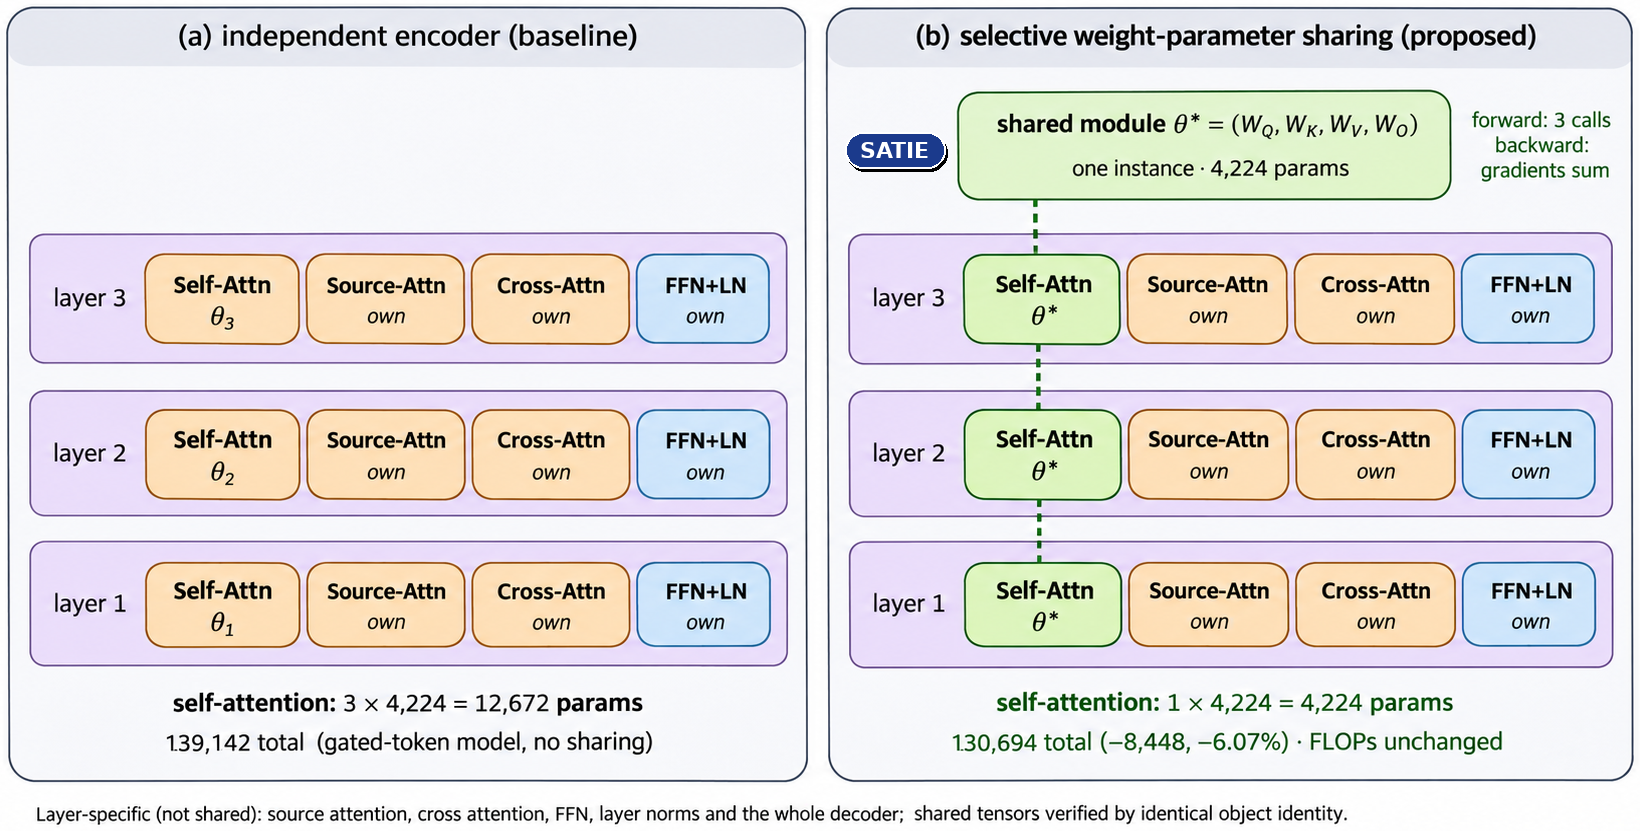
\includegraphics[width=0.85\textwidth]{figures/fig_sharing_new.png}
\caption{SATIE, selective weight-parameter sharing (\textbf{4}). (a)~Independent encoder: each of the three layers owns a self-attention module $\theta_l=(W_Q,W_K,W_V,W_O)$ (12,672 parameters in total). (b)~Proposed: one module $\theta^{\star}$ (4,224 parameters) is aliased in all three layers and receives the summed gradients; source attention, cross attention, feed-forward networks, layer norms and the decoder remain layer-specific. The total parameter count falls from 139,142 to 130,694 ($-6.07\%$) while FLOPs are unchanged.}
\label{fig:sharing}
\end{figure*}

\begin{algorithm}[t]
\caption{SATIE: encoder with selective self-attention sharing}\label{alg:share}
\begin{algorithmic}[1]
\Require embedded trajectory $\mathbf{x}^{(0)}$, speed tokens $\mathbf{m}^{(0)}\in\R^{15\times32}$; layers $N{=}3$
\Ensure trajectory memory $\mathbf{M}_{traj}$, speed stream $\mathbf{m}^{(N)}$
\State \textbf{construct:} $\mathrm{SA}^{\star}\gets\MHA(h{=}4,d{=}32)$ \Comment{single instance, 4,224 params}
\For{$l=1$ \textbf{to} $N$}
  \State $\mathrm{SA}^{(l)}\gets\mathrm{SA}^{\star}$ \Comment{alias, no copy}
  \State $\mathrm{SRC}^{(l)},\mathrm{CRS}^{(l)},\mathrm{FFN}^{(l)},\mathrm{LN}^{(l)}\gets$ new layer-specific modules
\EndFor
\For{$l=1$ \textbf{to} $N$}
  \State $\mathbf{x}'\gets\mathbf{x}^{(l-1)}+\Drop(\mathrm{SA}^{\star}(\LN(\mathbf{x}^{(l-1)})))$
  \State $\mathbf{m}'\gets\mathbf{m}^{(l-1)}+\Drop(\mathrm{SRC}^{(l)}(\LN(\mathbf{m}^{(l-1)}),\mathbf{x}'))$
  \State $\mathbf{x}''\gets\mathbf{x}'+\Drop(\mathrm{CRS}^{(l)}(\LN(\mathbf{x}'),\mathbf{m}'))$
  \State $(\mathbf{x}^{(l)},\mathbf{m}^{(l)})\gets\mathrm{FFN}^{(l)}\text{-residual blocks}(\mathbf{x}'',\mathbf{m}')$
\EndFor
\State \Return $\mathbf{x}^{(N)},\mathbf{m}^{(N)}$ \Comment{gradients of $\mathrm{SA}^{\star}$ sum over layers}
\end{algorithmic}
\end{algorithm}

\subsection{Decoder and Trajectory Prediction}\label{ssec:dec}
Each of the three decoder layers updates its query $Q^{(\ell)}\in\R^{45\times32}$ through three parallel attention branches whose outputs are summed (Fig.~\ref{fig:decoder}):
\begin{multline}
Q^{(\ell+1)}=\FFN\!\Big(A_M(Q^{(\ell)},\mathbf{M})+A_E(Q^{(\ell)},\mathbf{F}_{ego})\\+A_P(Q^{(\ell)},\mathbf{F}_{ped})\Big),
\end{multline}
with $d_{ff}{=}128$. The decoder has no self-attention. A linear head maps the last query to residual offsets $\Delta\mathbf{Y}\in\R^{45\times4}$, and the prediction is $\hat{\mathbf{Y}}=\Delta\mathbf{Y}+\mathbf{x}_T\mathbf{1}^\top$, i.e.\ a residual around constant-position extrapolation (Fig.~\ref{fig:overall}).

\begin{figure}[t]
\centering
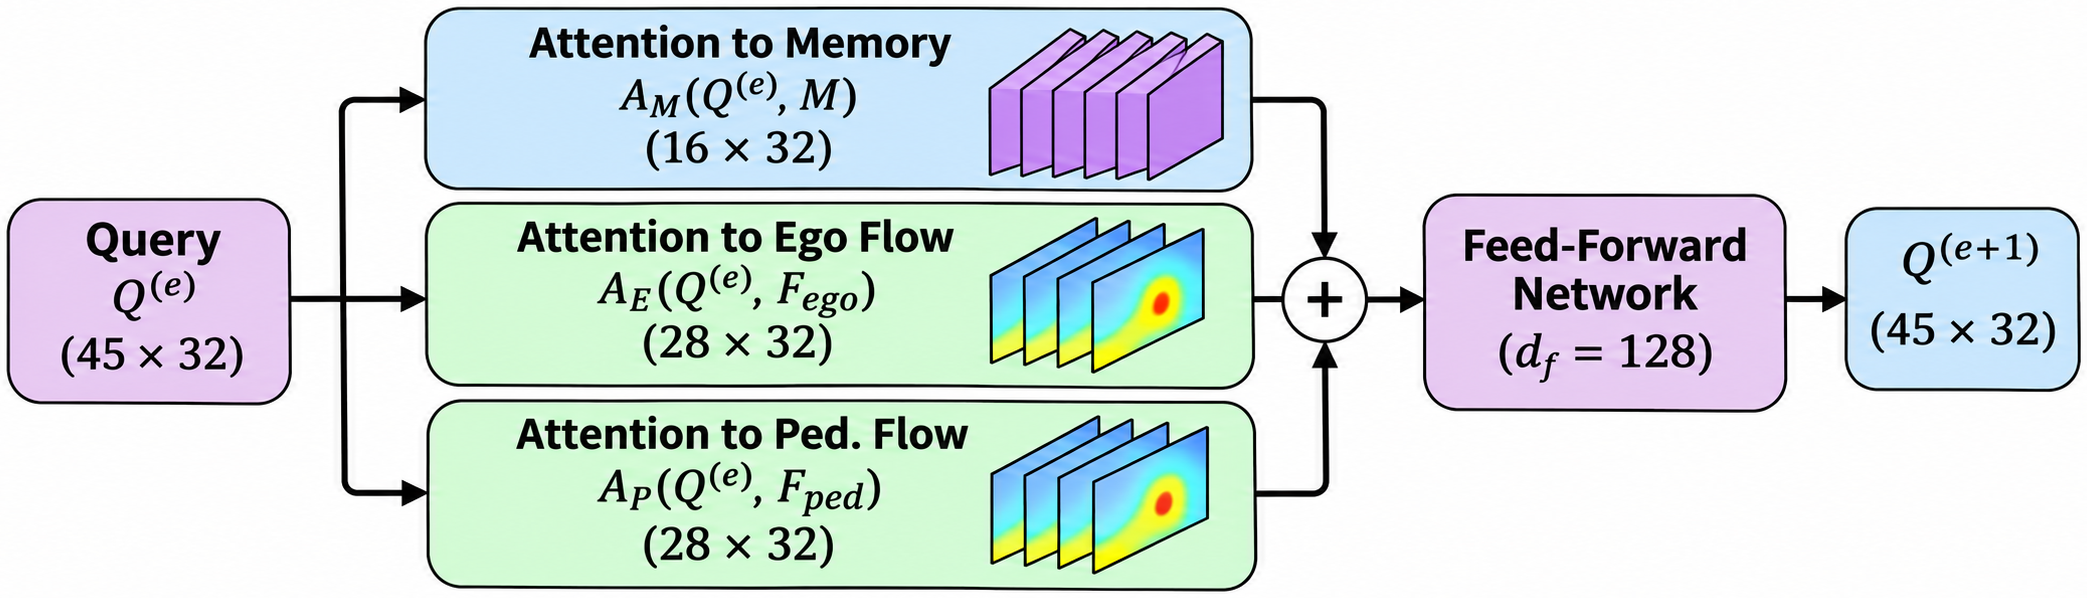
\includegraphics[width=\columnwidth]{figures/fig_decoder.png}
\caption{Decoder layer with three parallel attention sources: the augmented memory ($16{\times}32$), the ego-motion flow and the pedestrian flow (each $28{\times}32$), followed by a feed-forward network ($d_{ff}=128$).}
\label{fig:decoder}
\end{figure}

\subsection{Variants and Training}
\paragraph{Model variants.} Table~\ref{tab:budget} lists the models studied. \CAMTN integrates context through the admission-gated, memory-augmented token without sharing; \CAMTNS adds selective weight-parameter sharing and is the proposed final configuration. \DFMTN replaces the gated token with adaptive context-memory fusion (Sec.~\ref{ssec:fusion}), and \DFMTNS adds sharing to it. The adaptive-fusion models serve as the alternative realisation of the same design and are evaluated under the same protocol (Sec.~\ref{sec:ablation}).

\begin{table}[t]
\centering
\caption{Models studied and their exact parameter counts (measured by instantiating each model).}
\label{tab:budget}
\scriptsize
\begin{tabular}{p{5.6cm}r}
\toprule
Model & Parameters\\
\midrule
MTN (baseline) & 133,700\\
\CAMTN & 139,142\\
\CAMTNS (proposed) & 130,694\\
\DFMTN & 154,007\\
\DFMTNS & 145,559\\
\bottomrule
\end{tabular}
\end{table}

\paragraph{Training.} Every tensor with a matching shape is initialised from the official MTN checkpoint; new modules are randomly initialised and a tied module takes the first layer's weights. Training uses the Adam optimiser~\citep{kingma2015adam} (learning rate $10^{-3}$, batch size 8, one epoch) with an MSE loss between predicted and true 45-step boxes. No auxiliary loss is used.

\section{Experiments}\label{sec:results}

\subsection{Dataset}
The evaluation uses IDD-PeD~\citep{iddped2025}, a pedestrian dataset recorded in unstructured Indian traffic. It contains over 5,000 annotated pedestrians in continuous videos of 45\,s to 10\,min, a median ego speed of 30\,km/h, day and night scenes, per-track behavioural, scene and location annotations, and occlusion labels following the PIE convention. Compared with PIE and JAAD, pedestrians interact with dense traffic without lane discipline and signalisation is often absent, so motion-only trajectory predictors degrade strongly~\citep{iddped2025}. The official protocol uses a 70/30 train/test split, an observation window of 0.5\,s and a prediction horizon of 1.5\,s.

\subsection{Evaluation Metrics and Implementation Details}
All errors are in squared pixels. For predicted boxes $\hat{\mathbf{Y}}$ and ground truth $\mathbf{Y}$ over $H{=}45$ steps, with $\mathbf{c}_t$ the box centre,
\begin{align}
\mathrm{MSE}&=\tfrac1{4H}\textstyle\sum_{t=1}^{H}\|\hat{\mathbf{y}}_t-\mathbf{y}_t\|_2^2,\\
\mathrm{C\text{-}MSE}&=\tfrac1{2H}\textstyle\sum_{t=1}^{H}\|\hat{\mathbf{c}}_t-\mathbf{c}_t\|_2^2,\\
\mathrm{CF\text{-}MSE}&=\tfrac12\|\hat{\mathbf{c}}_H-\mathbf{c}_H\|_2^2,
\end{align}
where C-MSE is the centre MSE over all steps and CF-MSE the centre error at the final step (1.5\,s). The normalisation follows the evaluation routine of the implementation, which is identical for all models.

\paragraph{Matched proof-of-concept protocol.} All models in Table~\ref{tab:unified} use one fixed protocol: a 32/8/24 split of trajectories (training, validation, test), CPU Farneb\"ack optical flow~\citep{farneback2003}, the Adam optimiser with learning rate $10^{-3}$, batch size 8, an MSE loss, \emph{one epoch}, and three random seeds (20260928, 20260929, 20260930). Every tensor with a matching shape is initialised from the official MTN checkpoint. All models therefore see the same data, flow cache and initialisation, and differences can be attributed to the architecture and the seed. The test set consists of 24 held-out trajectories.\verify{number of held-out videos in the unified split} Parameter count and checkpoint size are also reported.

\subsection{Quantitative Results}
Table~\ref{tab:unified} lists the four evaluated models. \CAMTNS obtained the lowest mean MSE, C-MSE and CF-MSE and has the fewest parameters (130,694) and the smallest checkpoint. Relative to \CAMTN, it reduces MSE by $5.0\%$, C-MSE by $4.8\%$ and CF-MSE by $2.8\%$ (Table~\ref{tab:rel}). \DFMTN is worse than \CAMTN on every error metric and has $10.7\%$ more parameters; combining adaptive fusion with encoder self-attention sharing (\DFMTNS) recovers part of the loss on MSE and C-MSE but not on the final-step error.

\begin{table*}[t]
\centering
\caption{Matched comparison of the four models (mean $\pm$ standard deviation over three seeds; squared pixels, lower is better). The best value in each column is in bold.}
\label{tab:unified}
\scriptsize\setlength{\tabcolsep}{3pt}
\resizebox{0.92\textwidth}{!}{\begin{tabular}{p{6.6cm}rrrrr}
\toprule
Model & MSE & C-MSE & CF-MSE & Parameters & Checkpoint (MiB)\\
\midrule
PACE-Net without SATIE (SAGE + MASC) & 1137.11$\pm$20.16 & 1107.40$\pm$19.63 & 2971.36$\pm$103.13 & 139,142 & 1.85\\
PACE-Net (SAGE + MASC + SATIE) (proposed) & \textbf{1080.16$\pm$93.33} & \textbf{1053.83$\pm$95.13} & \textbf{2887.51$\pm$237.14} & \textbf{130,694} & \textbf{1.81}\\
PACE-Net with ROUTE & 1154.78$\pm$9.95 & 1124.20$\pm$10.08 & 3098.16$\pm$137.74 & 154,007 & 1.91\\
PACE-Net with ROUTE and SATIE & 1126.67$\pm$30.84 & 1098.43$\pm$27.25 & 3111.62$\pm$85.57 & 145,559 & 1.88\\
\bottomrule
\end{tabular}
}
\end{table*}

\begin{table}[t]
\centering
\caption{Change relative to \CAMTN, computed from the means of Table~\ref{tab:unified}.}
\label{tab:rel}
\scriptsize\setlength{\tabcolsep}{3pt}
\resizebox{\columnwidth}{!}{\begin{tabular}{p{4.3cm}rrrr}
\toprule
Model (relative to PACE-Net without SATIE (SAGE + MASC)) & $\Delta$MSE & $\Delta$C-MSE & $\Delta$CF-MSE & $\Delta$Params\\
\midrule
PACE-Net (SAGE + MASC + SATIE) & $-$5.01\% & $-$4.84\% & $-$2.82\% & $-$6.07\%\\
PACE-Net with ROUTE & +1.55\% & +1.52\% & +4.27\% & +10.68\%\\
PACE-Net with ROUTE and SATIE & $-$0.92\% & $-$0.81\% & +4.72\% & +4.61\%\\
\bottomrule
\end{tabular}
}
\end{table}

\begin{figure*}[t]
\centering
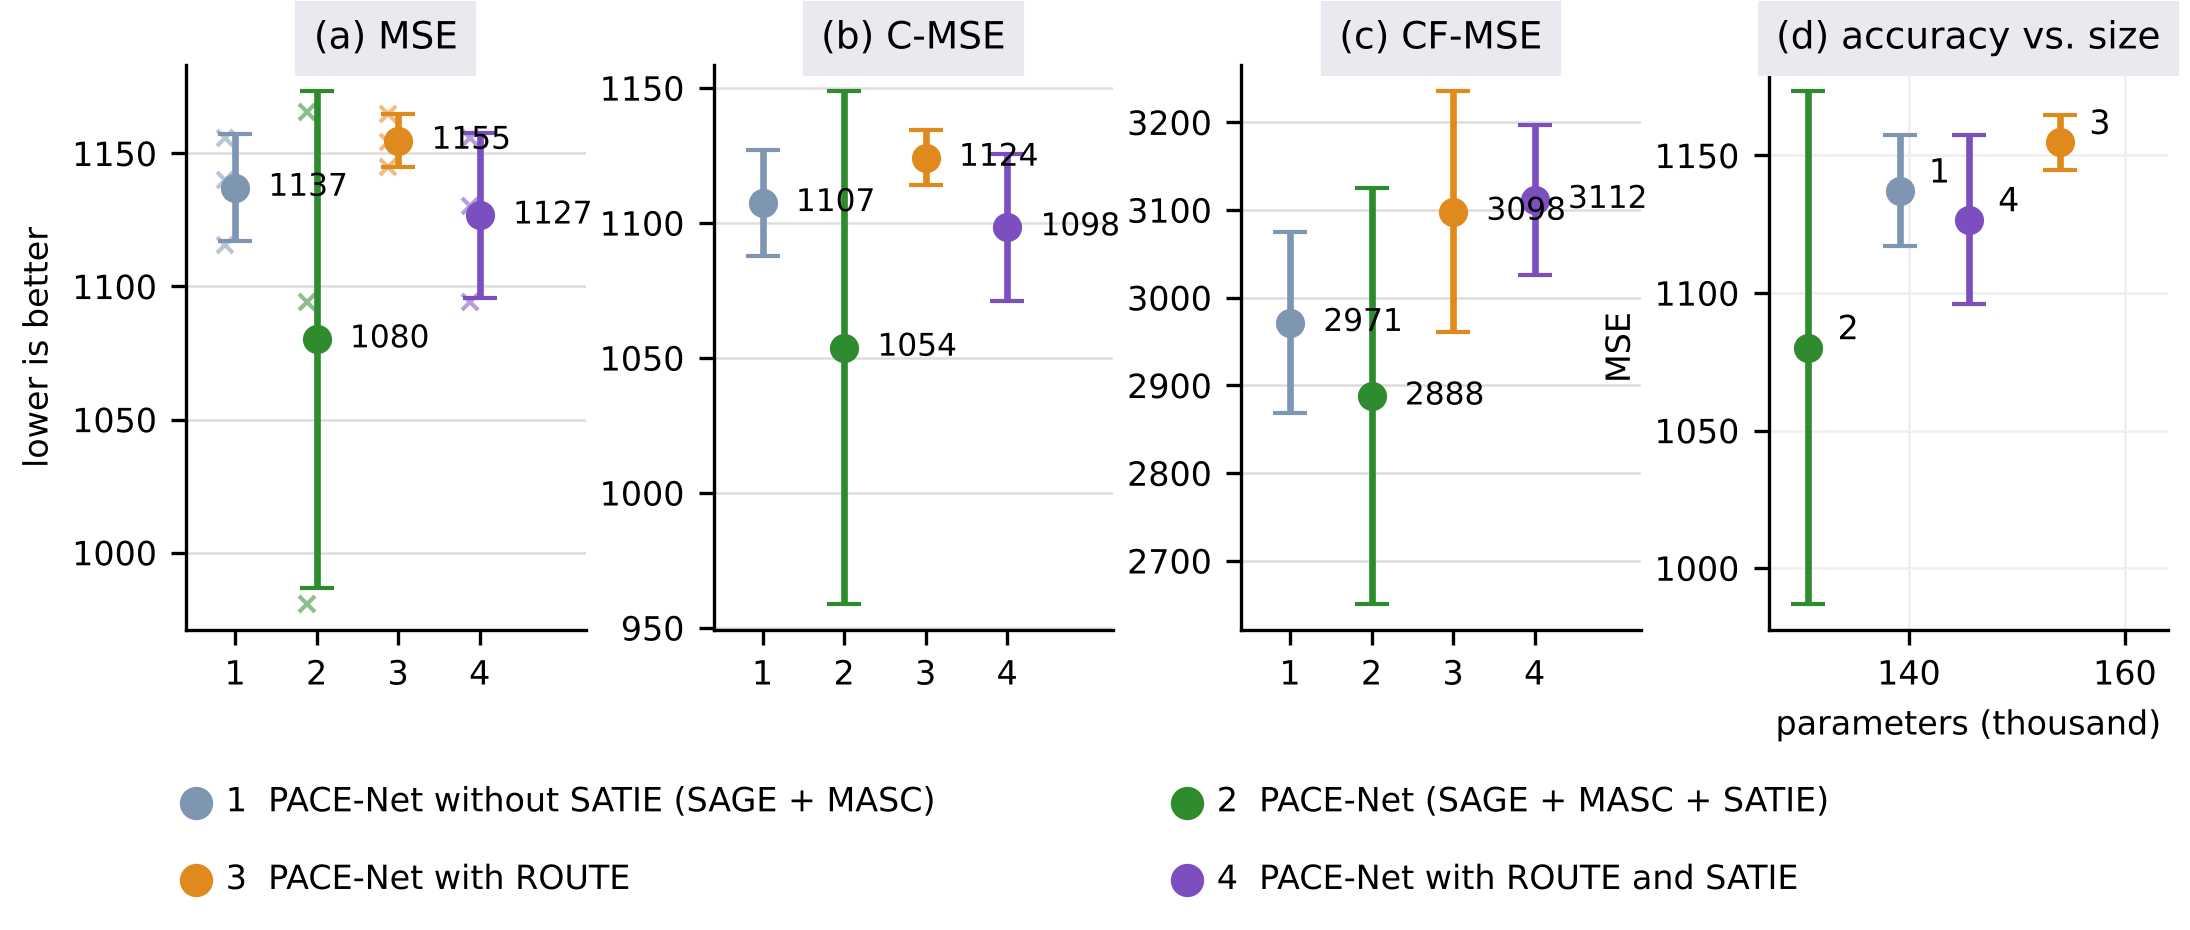
\includegraphics[width=0.92\textwidth]{figures/fig_results.png}
\caption{Test error of the four models. Crosses in panel (a) are individual seeds; dots and bars are mean $\pm$ standard deviation over three seeds. Panel (d) plots MSE against parameter count. Models are numbered as in the legend.}
\label{fig:results}
\end{figure*}

\paragraph{Seed-level behaviour.}
Table~\ref{tab:seed} and Fig.~\ref{fig:seeds} give the per-seed results. \CAMTNS is better than \CAMTN on two of three seeds (by 160 and 61) but worse on the third (by 50), so its standard deviation (93.3) is much larger than that of \CAMTN (20.2). A paired $t$-test over the three seeds gives $p=0.45$; \DFMTN and \DFMTNS are also not significantly different from \CAMTN ($p=0.24$ and $0.73$). The $5\%$ improvement is therefore regarded as a promising but unconfirmed trend. Its practical appeal is that comparable or lower error is obtained with $6\%$ fewer parameters, which is consistent with weight sharing acting as a regulariser in the short, small-data training regime used here.

\begin{table*}[t]
\centering
\caption{Per-seed test MSE and paired statistics against \CAMTN.}
\label{tab:seed}
\scriptsize\setlength{\tabcolsep}{3pt}
\resizebox{0.92\textwidth}{!}{\begin{tabular}{lrrrr}
\toprule
 & \multicolumn{1}{p{2.6cm}}{\raggedleft PACE-Net without SATIE (SAGE + MASC)} & \multicolumn{1}{p{3.4cm}}{\raggedleft PACE-Net (SAGE + MASC + SATIE)} & \multicolumn{1}{p{3cm}}{\raggedleft PACE-Net with ROUTE} & \multicolumn{1}{p{3.6cm}}{\raggedleft PACE-Net with ROUTE and SATIE}\\
Seed & & & &\\
\midrule
20260928 & 1140.10 & 980.57 & 1145.03 & 1094.26\\
20260929 & 1155.60 & 1094.30 & 1164.92 & 1130.09\\
20260930 & 1115.62 & 1165.62 & 1154.39 & 1155.65\\
\midrule
Mean $\pm$ std & 1137.11$\pm$20.16 & 1080.16$\pm$93.33 & 1154.78$\pm$9.95 & 1126.67$\pm$30.84\\
\midrule
Paired $\Delta$ vs.\ PACE-Net without SATIE (SAGE + MASC) (mean $\pm$ sd) & -- & $-$56.95$\pm$104.83 & +17.67$\pm$18.40 & $-$10.44$\pm$44.88\\
Seeds with lower error than PACE-Net without SATIE (SAGE + MASC) & -- & 2/3 & 0/3 & 2/3\\
Paired $t$-test $p$-value ($n{=}3$) & -- & 0.45 & 0.24 & 0.73\\
\bottomrule
\end{tabular}
}
\end{table*}

\begin{figure}[t]
\centering
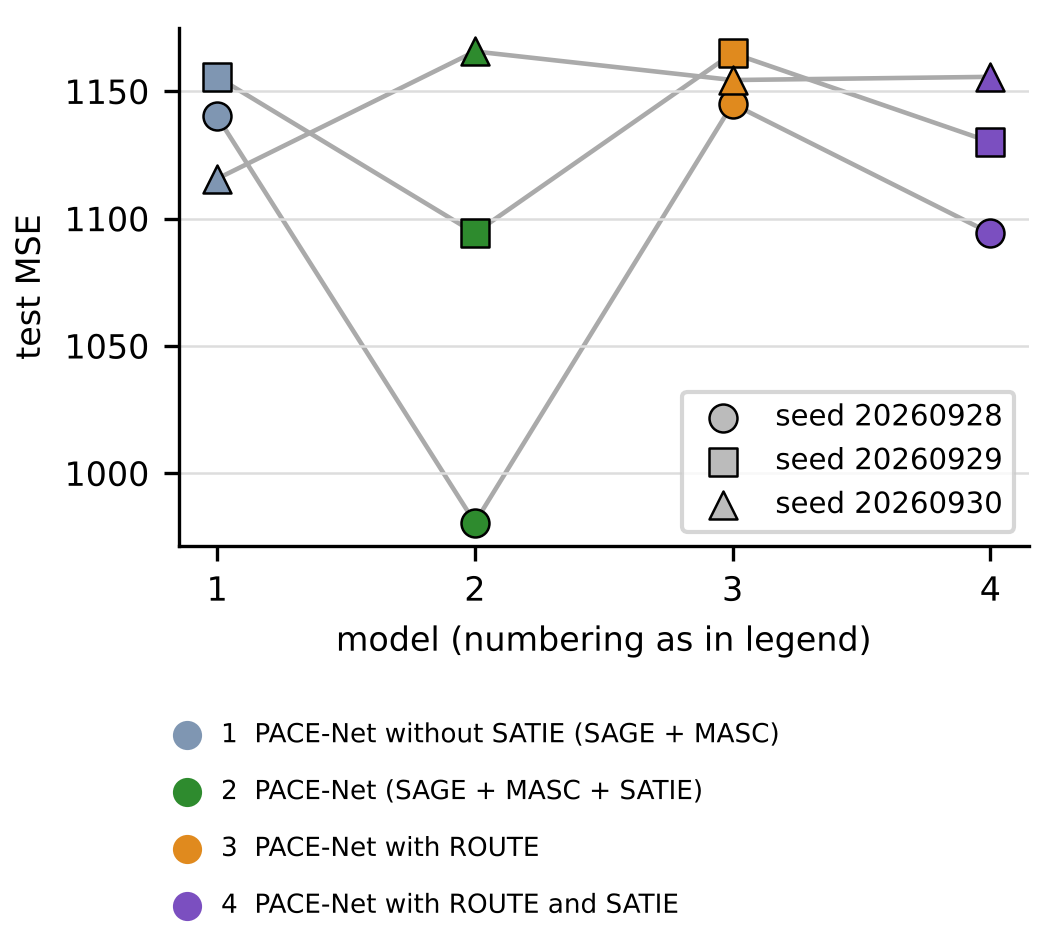
\includegraphics[width=\columnwidth]{figures/fig_seeds.png}
\caption{Per-seed test MSE of the four models; lines connect results obtained with the same seed. Models are numbered as in the legend.}
\label{fig:seeds}
\end{figure}

\paragraph{Computational cost.}
Encoder self-attention sharing reduces the number of unique parameters and the checkpoint size but not the amount of computation, since the three self-attention operations are still executed. The adaptive-fusion models evaluate all three fusion candidates before selecting one and are therefore both larger and no cheaper. Inference-time results are not reported, because timing on a shared CPU was too noisy to support a conclusion.

\paragraph{Effect of scene context.}
In an earlier single-seed study (12 epochs, 10 held-out trajectories of one video, the same CPU flow), adding the gated context token reduced MSE from 1242.98 to 1113.21 ($-10.4\%$), C-MSE from 1225.17 to 1094.57 and CF-MSE from 4093.85 to 3646.51 ($-10.9\%$). Because the protocol differs from Table~\ref{tab:unified} (training length, test set, number of seeds), these values are not directly comparable with it; re-running the baseline in the matched protocol is part of the planned work (Sec.~\ref{sec:limits}).

\subsection{Comparison with Prior Work}
Table~\ref{tab:prior} places the present results next to the published IDD-PeD trajectory benchmarks~\citep{iddped2025}: the deterministic PIETraj~\citep{rasouli2019pie} and MTN~\citep{yin2021mtn} and the stochastic BiTraP~\citep{yao2021bitrap} and SGNet~\citep{wang2022sgnet}, which report the best of 20 samples.

\begin{table}[t]
\centering
\caption{Comparison with published results (MSE, C-MSE, CF-MSE at 1.5\,s, squared pixels). Published rows are copied from Table~III of~\citep{iddped2025} (full test split, RAFT flow, GPU training). The rows for the present models use the reduced protocol described above and are therefore \emph{not directly comparable}.}
\label{tab:prior}
\scriptsize\resizebox{\columnwidth}{!}{%
\begin{tabular}{p{4.7cm}lrrr}
\toprule
Method & Type & MSE & C-MSE & CF-MSE\\
\midrule
PIETraj~\citep{rasouli2019pie} & deterministic & 2181 & 1979 & 8960\\
MTN~\citep{yin2021mtn} & deterministic & 1652 & 1489 & 6668\\
BiTraP~\citep{yao2021bitrap} & stochastic (best of 20) & 338 & 200 & 638\\
SGNet~\citep{wang2022sgnet} & stochastic (best of 20) & 310 & 190 & 531\\
\midrule
MTN, early single-seed study & deterministic & 1243 & 1225 & 4094\\
\CAMTN, early single-seed study & deterministic & 1113 & 1095 & 3647\\
\CAMTN, matched protocol & deterministic & 1137 & 1107 & 2971\\
\CAMTNS, matched protocol (proposed) & deterministic & 1080 & 1054 & 2888\\
\bottomrule
\end{tabular}}
\end{table}

\paragraph{Discussion.} Among deterministic methods, the published MTN reaches an MSE of 1652 on the official benchmark and PIETraj 2181; the context-aware models of this paper obtain 1080--1137 in the reduced protocol, which is in the same range as or below MTN, and the context token lowers the error relative to the motion-only baseline of the early study. The stochastic BiTraP and SGNet are about $3.5$--$5\times$ lower in MSE, as expected, because they report the best of 20 sampled futures and are goal-conditioned, whereas the proposed model outputs a single trajectory; closing this gap would require a multimodal output head, which is beyond the scope of this work. \textbf{These comparisons are indicative only}: the present numbers come from 24 trajectories, one training epoch and Farneb\"ack flow, whereas the published numbers use the entire 30\% test split, RAFT flow~\citep{teed2020raft} and fully trained GPU models. A fair claim of improvement over MTN requires re-running the baseline under exactly the same conditions as the proposed model, as described in Sec.~\ref{sec:ablation}.

\section{Ablation Study}\label{sec:ablation}
The proposed model has three separable ingredients: the scene information itself, the SAGE admission gate, and SATIE encoder self-attention sharing; ROUTE (adaptive context-memory fusion) is the alternative way of using the scene information. This section reports the ablations that have been executed and specifies the further ablations needed to attribute the gains to each component. Results from different protocols are never merged into one ranking; the matched four-model experiment is the primary comparison.

\subsection{Component Inventory}
\begin{table*}[t]
\centering
\caption{Components of the proposed model, the question each ablation answers, the comparison used, and its status.}
\label{tab:inventory}
\footnotesize
\begin{tabular}{p{3.6cm}p{5.6cm}p{5.6cm}p{2.4cm}}
\toprule
Component & Question & Comparison & Status\\
\midrule
Gated scene-context token & Does native scene and occlusion information help? & MTN vs.\ \CAMTN & done (single seed)\\
Context fields & Which of the six cues matter? & \CAMTN vs.\ \CAMTN without one field & proposed\\
SAGE admission gate & Is per-sample admission better than always adding the token? & Learned gate vs.\ always open vs.\ always closed & proposed\\
Gate relaxation & Does the discrete decision matter? & Hard Gumbel-softmax vs.\ sigmoid gate & proposed\\
Sharing scope & Which sub-modules can be tied safely? & None / decoder / encoder / encoder and decoder & done\\
SATIE (encoder self-attention sharing) & Does tying encoder self-attention help? & \CAMTN vs.\ \CAMTNS & done (three seeds)\\
ROUTE (adaptive context-memory fusion) & Is richer fusion better than a single token? & \CAMTN vs.\ \DFMTN & done (three seeds)\\
Interaction & Do sharing and fusion combine? & $2{\times}2$ factorial design & done\\
\bottomrule
\end{tabular}
\end{table*}

\subsection{Executed Ablations}
\paragraph{(1) Contribution of the scene-context branch.}
In the early paired study (one seed, 12 epochs, 10 held-out trajectories), MSE fell from 1242.98 (MTN) to 1113.21 (\CAMTN) and CF-MSE from 4093.85 to 3646.51 when the gated context token was added, at a cost of 5,442 parameters. This isolates the effect of the context token from sharing and fusion, but it rests on a single seed and a small test set.

\paragraph{(2) Scope of weight sharing.}
Sharing the complete encoder and decoder reduced the parameters of \CAMTN from 139,142 to 53,894 ($-61.3\%$) but raised MSE from 1113.21 to 1339.31 ($+20.3\%$) in its recorded study, so it was rejected: layers that play different roles should not be tied wholesale. Targeted sharing was then tested in a separate study (Table~\ref{tab:targeted}). Sharing decoder source-attention projections (in three variants) made MSE worse, whereas sharing the encoder self-attention was the only scope that improved on the unshared model of that study. Sharing decoder self-attention is impossible because the decoder has no self-attention, and head sharing requires a new projection parameterisation, so neither was run. The ordering suggests that sharing is harmless where the shared operation applies the same function repeatedly (encoder self-attention) and harmful where layers condition on different sources (decoder cross-attention).

\begin{table}[t]
\centering
\caption{Targeted-sharing study (separate protocol with its own unshared reference model; test MSE and final-step centre error CF-MSE, squared pixels).\verify{values transcribed from the earlier draft; not present in the evaluation workbook, confirm against run logs}}
\label{tab:targeted}
\scriptsize\resizebox{\columnwidth}{!}{%
\begin{tabular}{p{4.3cm}rrr}
\toprule
Shared parameters & Parameters & MSE & CF-MSE\\
\midrule
None (\CAMTN) & 139,142 & 972.51 & 2802.67\\
Decoder source-attention $Q,K,V,O$ & 130,694 & 1081.44 & 3369.58\\
Decoder source-attention $Q,K,V$ & 132,806 & 1188.92 & 3940.10\\
Decoder source-attention $K,V$ & 134,918 & 1152.49 & 3807.02\\
Encoder self-attention $Q,K,V,O$ (proposed) & 130,694 & 819.99 & 2441.16\\
\bottomrule
\end{tabular}}
\end{table}

\paragraph{(3) SATIE under the matched protocol.}
\CAMTNS lowers the mean MSE of \CAMTN by 56.9 ($-5.0\%$) and is better on two of three seeds, but the gap is not significant ($p=0.45$, $n=3$; Table~\ref{tab:seed}). The direction is consistent with the targeted-sharing study, which supports the claim that sharing does not hurt, whereas a confident claim of improvement needs more seeds.

\paragraph{(4) ROUTE and the factorial design.}
Table~\ref{tab:factorial} crosses the two design choices. Encoder self-attention sharing lowers the error in both rows ($-56.9$ for the gated context token and $-28.1$ with adaptive fusion), whereas adaptive fusion raises it in both columns ($+17.7$ without and $+46.5$ with sharing). The interaction is $+28.8$ MSE: sharing is less effective once fusion is added. The main effects are $-42.5$ (sharing) and $+32.1$ (fusion). The failure of adaptive fusion is therefore not caused by sharing. A plausible reason is that six extra tokens and a three-way gate introduce too many new parameters to be learned from very little training data in one epoch, and that the cross-attention candidate duplicates what the decoder's memory attention already does with a single token; this is a hypothesis that has not been tested.

\begin{table}[t]
\centering
\caption{$2{\times}2$ factorial ablation (mean test MSE over three seeds): use of context (gated token or adaptive fusion) $\times$ encoder self-attention sharing.}
\label{tab:factorial}
\scriptsize\resizebox{\columnwidth}{!}{\begin{tabular}{lrrr}
\toprule
Mean MSE (3 seeds) & Independent & Shared (SATIE) & Effect of\\
 & encoder self-attention & encoder self-attention & sharing\\
\midrule
SAGE + MASC (gated token) & 1137.11 & 1080.16 & $-$56.95\\
ROUTE (adaptive fusion) & 1154.78 & 1126.67 & $-$28.11\\
\midrule
Effect of ROUTE & +17.67 & +46.51 & \\
\bottomrule
\end{tabular}
}
\end{table}

\subsection{Ablations Still Required}
The executed ablations show that encoder self-attention sharing is not harmful and that adaptive fusion is not beneficial, but they do not yet isolate every part of the scene-context branch. The following experiments, all under the matched protocol, would complete the study.
\begin{enumerate}[leftmargin=1.6em,itemsep=1pt,topsep=2pt]
\item \textbf{Baseline in the matched protocol.} Train MTN (133,700 parameters) with three seeds to place MTN, \CAMTN and \CAMTNS on a common footing and to test the context effect statistically.
\item \textbf{Leave-one-out context fields.} Remove each of the six cues in turn (and all static labels together) to rank their contribution, e.g.\ whether occlusion alone explains most of the gain.
\item \textbf{Gate ablation.} Compare the learned gate with an always-open gate and an always-closed gate, and report the fraction of test samples admitted and the error on admitted versus rejected samples.
\item \textbf{Gate relaxation.} Compare the hard straight-through Gumbel-softmax gate with a soft sigmoid gate.
\item \textbf{Sharing granularity.} Share the projections in subsets (e.g.\ only $Q,K$), share only two of the three layers, and add two controls: independent weights with a shared initialisation, and a narrower unshared model with 130,694 parameters, to separate the regularising effect of tying from simple parameter reduction.
\item \textbf{More seeds and a larger test set.} At least ten seeds with a paired test and confidence interval, and evaluation on the full 30\% IDD-PeD test split.
\item \textbf{Stratified error analysis.} Report errors by occlusion state, day versus night, signalised versus unsignalised scenes and ego speed, as in the benchmark analysis of~\citep{iddped2025}.
\item \textbf{Training protocol.} Repeat the main comparison (MTN, \CAMTN, \CAMTNS) with RAFT optical flow and training to convergence, so that the results become comparable with the published numbers in Table~\ref{tab:prior}.
\end{enumerate}

\section{Limitations and Conclusion}\label{sec:limits}
\subsection{Limitations}
\begin{itemize}[leftmargin=1.4em,itemsep=1pt,topsep=2pt]
\item \textbf{Scale of the evaluation.} The matched experiment uses 24 test trajectories, three seeds and one training epoch with Farneb\"ack optical flow. The improvement of \CAMTNS over \CAMTN is within seed variance ($p=0.45$) and should be treated as a hypothesis for further testing.
\item \textbf{Not comparable with published benchmarks.} Published numbers use the full test split, RAFT flow and fully trained GPU models; no claim is made to outperform MTN, BiTraP or SGNet.
\item \textbf{Baseline not in the matched protocol.} The unmodified MTN was run only in the earlier single-seed study.
\item \textbf{Annotated context at inference.} The five static labels are IDD-PeD annotations of each track. In deployment they would have to be produced by a scene-understanding module, and its errors would propagate to the prediction.
\item \textbf{No reduction in computation.} Encoder self-attention sharing reduces parameters but not FLOPs, and the adaptive-fusion models evaluate all candidates before selecting one.
\item \textbf{Deterministic output.} The stochastic baselines report the best of 20 samples; a single-output model cannot match them without a multimodal output head.
\end{itemize}

\subsection{Conclusion}
This paper proposed PACE-Net (Pedestrian trajectory prediction with Admission-gated Context Enrichment), a dual-pathway architecture for pedestrian trajectory prediction in unstructured traffic, built on four components: ROUTE (adaptive context-memory fusion), SAGE (admission gating), MASC (memory augmentation with a gated native scene-context token) and SATIE (selective weight-parameter sharing). The gate can reject the context token per sample, in which case the decoder operates on the motion pathway alone, and SATIE removes $6.07\%$ of the parameters. In a matched three-seed proof-of-concept study on IDD-PeD, \CAMTNS had the lowest mean error, whereas ROUTE and wholesale weight sharing did not help. Because the evidence is limited in scale and the gain over \CAMTN is not statistically significant, the main value of the study lies in a reproducible design together with a set of controlled negative results. Confirming the effect on the full IDD-PeD split with RAFT optical flow and more seeds, together with the ablations of Sec.~\ref{sec:ablation}, is the immediate next step.

\bibliographystyle{plainnat}
\bibliography{references}
\end{document}
